So far, we have looked at statistical models of the form $Y\sim Normal(X\beta,\sigma\mathbbm{1})$. This is a flexible framework, allowing us to model linear and non-linear relationships between a response and predictors. We covered model formulation, model fitting, model checking, model selection, hypothesis test on model fits, predictions from models and the design of experiments to effectively collect data for statistical analysis. Today we will look at an even more general class of statistical models than linear models.

\subsection{Where linear models are not enough}

\begin{example}
	Consider yes/no outcomes or count data:
	
	\begin{center}
		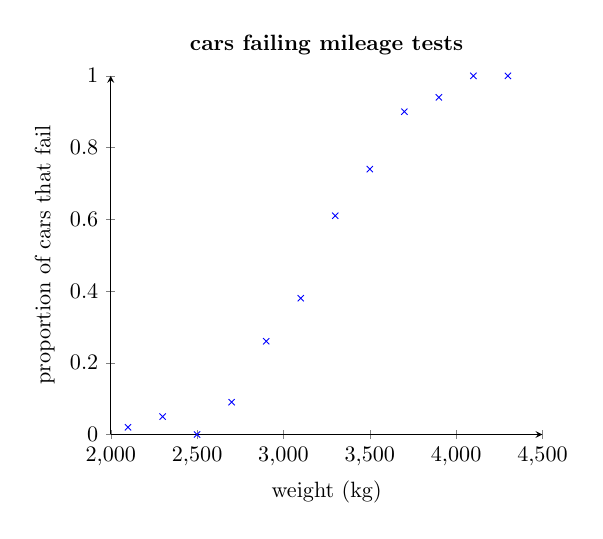
\begin{tikzpicture}[scale=0.8]
			\begin{axis}[
			xmin=2000, xmax=4500, xlabel=weight (kg),
			ymin=0, ymax=1, ylabel=proportion of cars that fail,
			title=\textbf{cars failing mileage tests},
			axis x line=bottom,
			axis y line=left,
			]
			\addplot[blue, only marks, mark=x] coordinates {
				(2100.00,0.02)
				(2300.00,0.05)
				(2500.00,0.00)
				(2700.00,0.09)
				(2900.00,0.26)
				(3100.00,0.38)
				(3300.00,0.61)
				(3500.00,0.74)
				(3700.00,0.90)
				(3900.00,0.94)
				(4100.00,1.00)
				(4300.00,1.00)
			};
			\end{axis}
		\end{tikzpicture}
		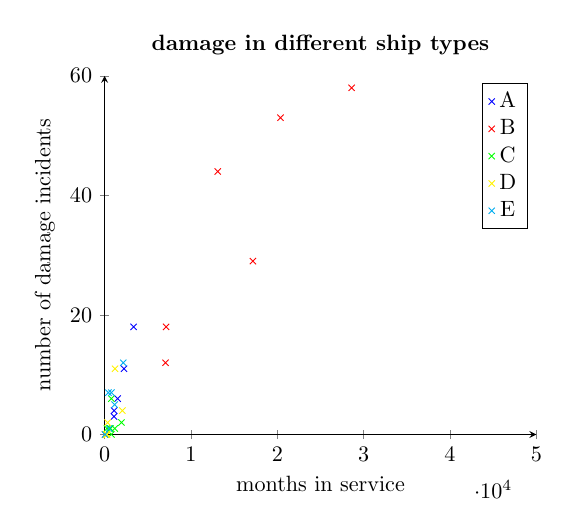
\begin{tikzpicture}[scale=0.8]
		\begin{axis}[
		xmin=0, xmax=50000, xlabel=months in service,
		ymin=0, ymax=60, ylabel=number of damage incidents,
		title=\textbf{damage in different ship types},
		axis x line=bottom,
		axis y line=left,
		]
		\addplot[blue, only marks, mark=x] coordinates {
			(127.00,0.00)
			(63.00,0.00)
			(1095.00,3.00)
			(1095.00,4.00)
			(1512.00,6.00)
			(3353.00,18.00)
			(2244.00,11.00)
		};
		\addlegendentry {A};
		\addplot[red, only marks, mark=x] coordinates {
			(44882.00,39.00)
			(17176.00,29.00)
			(28609.00,58.00)
			(20370.00,53.00)
			(7064.00,12.00)
			(13099.00,44.00)
			(7117.00,18.00)
		};
		\addlegendentry {B};
		\addplot[green, only marks, mark=x] coordinates {
			(1179.00,1.00)
			(552.00,1.00)
			(781.00,0.00)
			(676.00,1.00)
			(783.00,6.00)
			(1948.00,2.00)
			(274.00,1.00)
		};
		\addlegendentry {C};
		\addplot[yellow, only marks, mark=x] coordinates {
			(251.00,0.00)
			(105.00,0.00)
			(288.00,0.00)
			(192.00,0.00)
			(349.00,2.00)
			(1208.00,11.00)
			(2051.00,4.00)
		};
		\addlegendentry {D};
		\addplot[cyan, only marks, mark=x] coordinates {
			(45.00,0.00)
			(789.00,7.00)
			(437.00,7.00)
			(1157.00,5.00)
			(2161.00,12.00)
			(542.00,1.00)
		};
		\addlegendentry {E};
		\end{axis}
		\end{tikzpicture}
	\end{center}
	
	The normal distribution for the errors $\epsilon$ is not appropriate here.
\end{example}

There is a more general class of models than linear models, called \begriff{Generalised Linear Models} (GLMs). They can be written as
\begin{align}
	\mathbb{E}(Y_i) &\equiv \mu_i =\gamma(X_i\beta) \notag \\
	Y_i &\overset{\text{independent}}{\sim} \text{ Exponential family distribution} \notag
\end{align}
where $\gamma$ is any smooth monotonic function. The Exponential family of distributions includes distributions such as Poisson, Gaussian, binomial and gamma.

GLMs are written in terms of the \begriff{link function}, $g$, which is the inverse of $\gamma$:
\begin{align}
	g(\mu_i) &= X_i\beta \notag \\
	Y_i &\overset{\text{independent}}{\sim} \text{ Exponential family distribution} \notag
\end{align}

\begin{example}
	\begin{align}
		Y_i &\sim \text{Binomial} \notag \\
		g(\mu) &= \ln\left(\frac{\mu}{1-\mu}\right)\notag
	\end{align}
	logit link function.
\end{example}

\begin{example}
	Linear models are a special case of GLMs.
\end{example}

The link functions in the following table are only examples. Other link functions can be used with distributions.
\begin{center}
	\begin{tabular}{c|c|c|c|c}
		\textbf{distribution} & \textbf{support} & \text{use} & \textbf{link name} & \textbf{link function} \\
		\hline
		normal & $(-\infty,\infty)$ & linear response & identity & $\mu$ \\
		exponential & $(0,\infty)$ & exponential response & inverse & $\mu^{-1}$ \\
		gamma & $(0,\infty)$ & gamma response & log & $\ln(\mu)$ \\
		Poisson & $\natur_0$ & count data & log & $\ln(\mu)$ \\
		binomial & & proportions of yes/no occurrences & logit & $\ln\left(\frac{\mu}{1-\mu}\right)$
	\end{tabular}
\end{center}

\begin{example}
	AIDS cases per year in Belgium at the start of the epidemic
	\begin{center}
		\begin{tikzpicture}
			\begin{axis}[
			xmin=0, xmax=13, xlabel=year since 1980,
			ymin=0, ymax=250, ylabel=new AIDS cases,
			axis x line=bottom,
			axis y line=left,
			]
			\addplot[blue, only marks, mark=x] coordinates {
				(1,10)
				(2,15)
				(3,30)
				(4,55)
				(5,65)
				(6,70)
				(7,130)
				(8,150)
				(9,170)
				(10,210)
				(11,250)
				(12,245)
				(13,240)
			};
			\end{axis}
		\end{tikzpicture}
	\end{center}
	Early in an epidemic, an exponential increase in cases can occur
	\begin{align}
		\mathbb{E}(Y_i) &\equiv \mu_i = \delta\exp(\alpha t_i) \notag \\
		Y_i &\sim Poisson(\mu_i) \notag
	\end{align}
	Taking the logarithm of both sides and letting $\beta_0\equiv\log(\delta)$ and $\beta_1\equiv\alpha$
	\begin{align}
		\log(\mu_i) &= \beta_0 + \beta_1 t_i \notag \\
		Y_i &\sim Poisson(\mu_i) \notag
	\end{align}
	which is a GLM with a log link.
\end{example}

\subsection{Model fitting in GLMs}

To fit GLMs to data, we use the principle of Maximum Likelihood Estimation (MLE). Given parameters $\beta$, we can write down $f(Y\mid \beta)$, the probability or probability density function of the response $Y$. For observed data, $Y_i^{\text{obs}}$, the likelihood function is
\begin{align}
	L(\beta) = \prod_i f(Y_i^{\text{obs}}\mid \beta)\notag
\end{align}
For GLMs, there is no closed form solution for the values of $\beta$ that maximise this function. Instead, MLE is performed numerically, using a technique called \begriff{iteratively re-weighted least squares} (IRLS). In principle, other optimisation algorithms could also be used for MLE.

\begin{example}[logistic regression]
	The proportion of cars of various weights that fail a mileage test.
	
	\begin{center}
		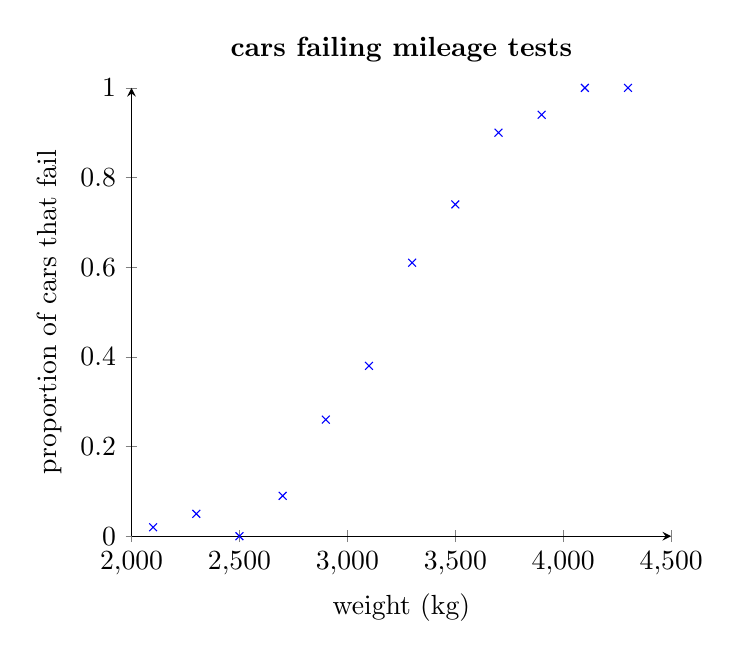
\begin{tikzpicture}
		\begin{axis}[
		xmin=2000, xmax=4500, xlabel=weight (kg),
		ymin=0, ymax=1, ylabel=proportion of cars that fail,
		title=\textbf{cars failing mileage tests},
		axis x line=bottom,
		axis y line=left,
		]
		\addplot[blue, only marks, mark=x] coordinates {
			(2100.00,0.02)
			(2300.00,0.05)
			(2500.00,0.00)
			(2700.00,0.09)
			(2900.00,0.26)
			(3100.00,0.38)
			(3300.00,0.61)
			(3500.00,0.74)
			(3700.00,0.90)
			(3900.00,0.94)
			(4100.00,1.00)
			(4300.00,1.00)
		};
		\end{axis}
		\end{tikzpicture}
	\end{center}
	
	Data are bounded, so LM is not appropriate and we fit a GLM with
	\begin{align}
		Y_i &\sim Binomial(\mu_i) \notag \\
		g(\mu_i) &= X_i\beta = \beta_0 + \beta_1\cdot weight_i \notag
	\end{align}
	Here $g(\mu_i) = \ln\left(\frac{\mu_i}{1-\mu_i}\right)$, so $\mu_i=\frac{1}{1+\exp(-X_i\beta)}$, the logistic function.
\end{example}

\subsection{GLM assumptions and checking}

Important GLM assumptions:
\begin{itemize}
	\item Independence
	\item Distributional assumptions
	\item Weak exogeneity
	\item Linear relationship between transformed response and predictors (link function)
\end{itemize}
Residual plots are still useful to check if model assumptions hold.

As we use different distributions, we cannot simply use raw residuals, as for linear models. Two common types of residuals that attempt to mimic behaviour of residuals for LMs:
\begin{itemize}
	\item \person{Pearson} Residuals
	\item Deviance Residuals
\end{itemize}

Residual plots using deviance residuals.

\begin{center}
	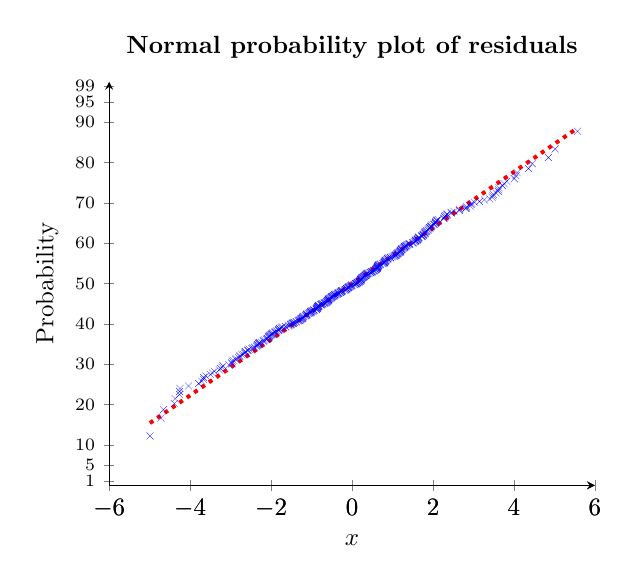
\begin{tikzpicture}[scale=0.9]
	\begin{axis}[
	xmin=-6, xmax=6, xlabel=$x$,
	ymin=-4, ymax=4, ylabel=$y$,
	samples=400,
	axis x line=bottom,
	axis y line=none,
	domain=-6:-6,
	title=\textbf{Normal probability plot of residuals}
	]
	\addplot[mark=x,blue, only marks, ultra thin] coordinates {
		(-4.99,-3.02)
		(-4.72,-2.67)
		(-4.66,-2.50)
		(-4.39,-2.38)
		(-4.37,-2.28)
		(-4.26,-2.20)
		(-4.26,-2.14)
		(-4.25,-2.08)
		(-4.04,-2.03)
		(-3.79,-1.98)
		(-3.71,-1.94)
		(-3.67,-1.90)
		(-3.67,-1.86)
		(-3.61,-1.83)
		(-3.50,-1.80)
		(-3.45,-1.77)
		(-3.40,-1.74)
		(-3.28,-1.71)
		(-3.25,-1.68)
		(-3.21,-1.66)
		(-3.19,-1.63)
		(-3.04,-1.61)
		(-2.97,-1.59)
		(-2.97,-1.57)
		(-2.96,-1.54)
		(-2.94,-1.52)
		(-2.88,-1.50)
		(-2.86,-1.49)
		(-2.80,-1.47)
		(-2.77,-1.45)
		(-2.77,-1.43)
		(-2.72,-1.41)
		(-2.69,-1.40)
		(-2.65,-1.38)
		(-2.64,-1.36)
		(-2.63,-1.35)
		(-2.58,-1.33)
		(-2.57,-1.32)
		(-2.54,-1.30)
		(-2.47,-1.29)
		(-2.45,-1.27)
		(-2.41,-1.26)
		(-2.35,-1.25)
		(-2.35,-1.23)
		(-2.34,-1.22)
		(-2.33,-1.21)
		(-2.31,-1.19)
		(-2.30,-1.18)
		(-2.28,-1.17)
		(-2.24,-1.16)
		(-2.19,-1.14)
		(-2.19,-1.13)
		(-2.16,-1.12)
		(-2.11,-1.11)
		(-2.10,-1.10)
		(-2.09,-1.09)
		(-2.07,-1.07)
		(-2.06,-1.06)
		(-2.05,-1.05)
		(-2.04,-1.04)
		(-2.03,-1.03)
		(-2.01,-1.02)
		(-1.99,-1.01)
		(-1.98,-1.00)
		(-1.97,-0.99)
		(-1.96,-0.98)
		(-1.91,-0.97)
		(-1.90,-0.96)
		(-1.88,-0.95)
		(-1.86,-0.94)
		(-1.82,-0.93)
		(-1.81,-0.92)
		(-1.81,-0.91)
		(-1.79,-0.90)
		(-1.79,-0.89)
		(-1.75,-0.88)
		(-1.73,-0.87)
		(-1.72,-0.86)
		(-1.64,-0.86)
		(-1.64,-0.85)
		(-1.57,-0.84)
		(-1.56,-0.83)
		(-1.52,-0.82)
		(-1.52,-0.81)
		(-1.50,-0.80)
		(-1.47,-0.79)
		(-1.45,-0.78)
		(-1.45,-0.78)
		(-1.42,-0.77)
		(-1.38,-0.76)
		(-1.38,-0.75)
		(-1.33,-0.74)
		(-1.31,-0.73)
		(-1.31,-0.73)
		(-1.28,-0.72)
		(-1.27,-0.71)
		(-1.26,-0.70)
		(-1.25,-0.69)
		(-1.23,-0.69)
		(-1.22,-0.68)
		(-1.22,-0.67)
		(-1.21,-0.66)
		(-1.21,-0.65)
		(-1.19,-0.65)
		(-1.15,-0.64)
		(-1.14,-0.63)
		(-1.13,-0.62)
		(-1.12,-0.62)
		(-1.12,-0.61)
		(-1.11,-0.60)
		(-1.08,-0.59)
		(-1.06,-0.59)
		(-1.04,-0.58)
		(-1.02,-0.57)
		(-1.02,-0.56)
		(-1.01,-0.56)
		(-1.01,-0.55)
		(-0.99,-0.54)
		(-0.96,-0.54)
		(-0.94,-0.53)
		(-0.94,-0.52)
		(-0.89,-0.51)
		(-0.88,-0.51)
		(-0.88,-0.50)
		(-0.87,-0.49)
		(-0.86,-0.49)
		(-0.86,-0.48)
		(-0.85,-0.47)
		(-0.85,-0.46)
		(-0.84,-0.46)
		(-0.83,-0.45)
		(-0.83,-0.44)
		(-0.82,-0.44)
		(-0.82,-0.43)
		(-0.77,-0.42)
		(-0.76,-0.42)
		(-0.75,-0.41)
		(-0.74,-0.40)
		(-0.72,-0.40)
		(-0.69,-0.39)
		(-0.67,-0.38)
		(-0.65,-0.38)
		(-0.63,-0.37)
		(-0.62,-0.36)
		(-0.62,-0.36)
		(-0.62,-0.35)
		(-0.60,-0.34)
		(-0.60,-0.34)
		(-0.59,-0.33)
		(-0.58,-0.32)
		(-0.58,-0.32)
		(-0.58,-0.31)
		(-0.57,-0.30)
		(-0.55,-0.30)
		(-0.54,-0.29)
		(-0.52,-0.28)
		(-0.51,-0.28)
		(-0.51,-0.27)
		(-0.50,-0.26)
		(-0.48,-0.26)
		(-0.47,-0.25)
		(-0.45,-0.24)
		(-0.44,-0.24)
		(-0.43,-0.23)
		(-0.43,-0.22)
		(-0.42,-0.22)
		(-0.40,-0.21)
		(-0.36,-0.21)
		(-0.36,-0.20)
		(-0.35,-0.19)
		(-0.34,-0.19)
		(-0.32,-0.18)
		(-0.29,-0.17)
		(-0.28,-0.17)
		(-0.27,-0.16)
		(-0.26,-0.15)
		(-0.26,-0.15)
		(-0.25,-0.14)
		(-0.24,-0.14)
		(-0.19,-0.13)
		(-0.17,-0.12)
		(-0.16,-0.12)
		(-0.14,-0.11)
		(-0.13,-0.10)
		(-0.13,-0.10)
		(-0.11,-0.09)
		(-0.10,-0.08)
		(-0.09,-0.08)
		(-0.09,-0.07)
		(-0.08,-0.07)
		(-0.07,-0.06)
		(-0.04,-0.05)
		(-0.03,-0.05)
		(-0.02,-0.04)
		(-0.01,-0.03)
		(-0.00,-0.03)
		(0.05,-0.02)
		(0.07,-0.02)
		(0.09,-0.01)
		(0.09,-0.00)
		(0.11,0.00)
		(0.13,0.01)
		(0.13,0.02)
		(0.14,0.02)
		(0.16,0.03)
		(0.17,0.03)
		(0.18,0.04)
		(0.19,0.05)
		(0.20,0.05)
		(0.20,0.06)
		(0.21,0.07)
		(0.22,0.07)
		(0.22,0.08)
		(0.22,0.08)
		(0.23,0.09)
		(0.23,0.10)
		(0.23,0.10)
		(0.24,0.11)
		(0.25,0.12)
		(0.27,0.12)
		(0.28,0.13)
		(0.29,0.14)
		(0.30,0.14)
		(0.31,0.15)
		(0.31,0.15)
		(0.33,0.16)
		(0.33,0.17)
		(0.35,0.17)
		(0.35,0.18)
		(0.36,0.19)
		(0.37,0.19)
		(0.38,0.20)
		(0.40,0.21)
		(0.43,0.21)
		(0.46,0.22)
		(0.47,0.22)
		(0.49,0.23)
		(0.49,0.24)
		(0.50,0.24)
		(0.53,0.25)
		(0.54,0.26)
		(0.55,0.26)
		(0.58,0.27)
		(0.58,0.28)
		(0.58,0.28)
		(0.60,0.29)
		(0.60,0.30)
		(0.62,0.30)
		(0.62,0.31)
		(0.62,0.32)
		(0.63,0.32)
		(0.63,0.33)
		(0.63,0.34)
		(0.64,0.34)
		(0.64,0.35)
		(0.65,0.36)
		(0.66,0.36)
		(0.66,0.37)
		(0.67,0.38)
		(0.70,0.38)
		(0.70,0.39)
		(0.75,0.40)
		(0.78,0.40)
		(0.79,0.41)
		(0.80,0.42)
		(0.80,0.42)
		(0.80,0.43)
		(0.80,0.44)
		(0.82,0.44)
		(0.82,0.45)
		(0.83,0.46)
		(0.83,0.46)
		(0.85,0.47)
		(0.86,0.48)
		(0.88,0.49)
		(0.88,0.49)
		(0.88,0.50)
		(0.90,0.51)
		(0.95,0.51)
		(0.95,0.52)
		(0.99,0.53)
		(1.01,0.54)
		(1.04,0.54)
		(1.05,0.55)
		(1.07,0.56)
		(1.08,0.56)
		(1.09,0.57)
		(1.10,0.58)
		(1.11,0.59)
		(1.13,0.59)
		(1.13,0.60)
		(1.14,0.61)
		(1.16,0.62)
		(1.18,0.62)
		(1.19,0.63)
		(1.19,0.64)
		(1.20,0.65)
		(1.20,0.65)
		(1.20,0.66)
		(1.22,0.67)
		(1.22,0.68)
		(1.23,0.69)
		(1.24,0.69)
		(1.26,0.70)
		(1.28,0.71)
		(1.29,0.72)
		(1.30,0.73)
		(1.30,0.73)
		(1.32,0.74)
		(1.33,0.75)
		(1.35,0.76)
		(1.37,0.77)
		(1.40,0.78)
		(1.41,0.78)
		(1.43,0.79)
		(1.50,0.80)
		(1.50,0.81)
		(1.52,0.82)
		(1.55,0.83)
		(1.57,0.84)
		(1.57,0.85)
		(1.57,0.86)
		(1.60,0.86)
		(1.62,0.87)
		(1.62,0.88)
		(1.63,0.89)
		(1.64,0.90)
		(1.65,0.91)
		(1.65,0.92)
		(1.72,0.93)
		(1.73,0.94)
		(1.73,0.95)
		(1.76,0.96)
		(1.76,0.97)
		(1.77,0.98)
		(1.80,0.99)
		(1.80,1.00)
		(1.80,1.01)
		(1.80,1.02)
		(1.82,1.03)
		(1.84,1.04)
		(1.85,1.05)
		(1.88,1.06)
		(1.88,1.07)
		(1.90,1.09)
		(1.92,1.10)
		(1.92,1.11)
		(1.94,1.12)
		(1.95,1.13)
		(1.95,1.14)
		(1.97,1.16)
		(2.02,1.17)
		(2.03,1.18)
		(2.06,1.19)
		(2.06,1.21)
		(2.07,1.22)
		(2.07,1.23)
		(2.09,1.25)
		(2.10,1.26)
		(2.13,1.27)
		(2.26,1.29)
		(2.28,1.30)
		(2.29,1.32)
		(2.29,1.33)
		(2.31,1.35)
		(2.34,1.36)
		(2.35,1.38)
		(2.45,1.40)
		(2.45,1.41)
		(2.52,1.43)
		(2.65,1.45)
		(2.66,1.47)
		(2.81,1.49)
		(2.82,1.50)
		(2.83,1.52)
		(2.92,1.54)
		(2.94,1.57)
		(2.96,1.59)
		(3.03,1.61)
		(3.15,1.63)
		(3.27,1.66)
		(3.40,1.68)
		(3.46,1.71)
		(3.48,1.74)
		(3.49,1.77)
		(3.56,1.80)
		(3.61,1.83)
		(3.62,1.86)
		(3.63,1.90)
		(3.72,1.94)
		(3.76,1.98)
		(3.82,2.03)
		(4.01,2.08)
		(4.05,2.14)
		(4.08,2.20)
		(4.36,2.28)
		(4.45,2.38)
		(4.85,2.50)
		(5.02,2.67)
		(5.57,3.02)
	};
	\addplot[dotted,red,ultra thick] coordinates {
		(-4.9938,-2.7658)
		(5.5747,3.0865)
	};
	\end{axis}
	\begin{axis}[
	xmin=-6,
	xmax=6,
	ymin=0,
	ymax=100,
	ylabel=Probability,
	axis y line=left,
	axis x line=bottom,
	yticklabel style={font=\scriptsize},
	ytick={1,5,10,20,30,40,50,60,70,80,90,95,99},
	]
	\end{axis}
	\end{tikzpicture}
	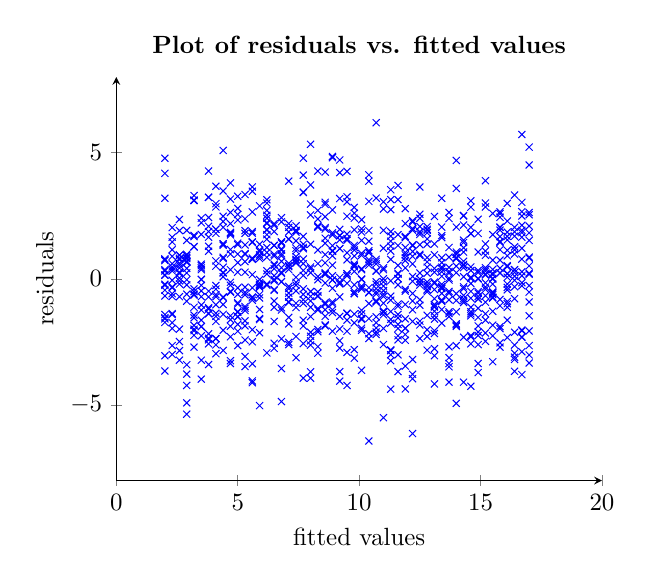
\begin{tikzpicture}[scale=0.9]
	\begin{axis}[
	xmin=0, xmax=20, xlabel=fitted values,
	ymin=-8, ymax=8, ylabel=residuals,
	samples=400,
	axis x line=bottom,
	axis y line=left,
	domain=0:20,
	title=\textbf{Plot of residuals vs. fitted values}
	]
	\addplot[mark=x,blue, only marks] coordinates {
		(2.00,-0.26)
		(2.00,-1.54)
		(2.00,4.78)
		(2.00,0.15)
		(2.00,0.75)
		(2.00,0.79)
		(2.00,-0.22)
		(2.00,-3.66)
		(2.00,4.18)
		(2.00,0.72)
		(2.00,-1.59)
		(2.00,-0.45)
		(2.00,3.19)
		(2.00,0.31)
		(2.00,0.36)
		(2.00,-0.68)
		(2.00,-3.05)
		(2.00,-1.42)
		(2.00,-1.73)
		(2.00,0.14)
		(2.30,0.31)
		(2.30,-0.36)
		(2.30,1.46)
		(2.30,-0.70)
		(2.30,0.47)
		(2.30,-1.74)
		(2.30,-1.97)
		(2.30,-0.59)
		(2.30,1.65)
		(2.30,0.39)
		(2.30,0.60)
		(2.30,-1.42)
		(2.30,-1.38)
		(2.30,1.15)
		(2.30,0.89)
		(2.30,-2.65)
		(2.30,-3.00)
		(2.30,2.03)
		(2.30,-0.06)
		(2.30,-0.32)
		(2.60,0.76)
		(2.60,-0.21)
		(2.60,0.43)
		(2.60,0.94)
		(2.60,-3.23)
		(2.60,0.03)
		(2.60,-0.08)
		(2.60,0.81)
		(2.60,0.61)
		(2.60,-2.49)
		(2.60,0.26)
		(2.60,-2.00)
		(2.60,-0.71)
		(2.60,0.21)
		(2.60,1.91)
		(2.60,0.93)
		(2.60,0.53)
		(2.60,-2.85)
		(2.60,0.22)
		(2.60,2.35)
		(2.90,-4.23)
		(2.90,0.92)
		(2.90,-4.92)
		(2.90,-0.61)
		(2.90,0.80)
		(2.90,-3.41)
		(2.90,1.52)
		(2.90,0.41)
		(2.90,1.92)
		(2.90,0.97)
		(2.90,-0.89)
		(2.90,0.65)
		(2.90,-0.04)
		(2.90,-3.78)
		(2.90,0.68)
		(2.90,0.68)
		(2.90,0.85)
		(2.90,0.23)
		(2.90,-0.24)
		(2.90,-5.37)
		(3.20,3.10)
		(3.20,-1.85)
		(3.20,-1.44)
		(3.20,1.67)
		(3.20,-1.13)
		(3.20,-2.00)
		(3.20,1.28)
		(3.20,-0.51)
		(3.20,-2.24)
		(3.20,3.30)
		(3.20,-0.61)
		(3.20,-1.55)
		(3.20,-2.71)
		(3.20,-0.65)
		(3.20,3.11)
		(3.20,1.26)
		(3.20,-2.06)
		(3.20,-0.40)
		(3.20,1.72)
		(3.20,3.12)
		(3.50,-0.26)
		(3.50,-1.64)
		(3.50,0.58)
		(3.50,-2.26)
		(3.50,1.76)
		(3.50,-1.89)
		(3.50,-1.24)
		(3.50,-3.98)
		(3.50,-1.90)
		(3.50,0.52)
		(3.50,2.40)
		(3.50,2.22)
		(3.50,-3.23)
		(3.50,-0.71)
		(3.50,-0.02)
		(3.50,-0.03)
		(3.50,0.43)
		(3.50,0.36)
		(3.50,-1.04)
		(3.50,-0.48)
		(3.80,-1.39)
		(3.80,-1.37)
		(3.80,1.87)
		(3.80,-2.42)
		(3.80,-0.72)
		(3.80,-2.36)
		(3.80,1.29)
		(3.80,-2.18)
		(3.80,-3.40)
		(3.80,-2.58)
		(3.80,1.09)
		(3.80,4.27)
		(3.80,-1.15)
		(3.80,1.65)
		(3.80,3.23)
		(3.80,2.43)
		(3.80,3.23)
		(3.80,-1.20)
		(3.80,2.08)
		(3.80,-0.49)
		(4.10,-2.97)
		(4.10,-0.71)
		(4.10,0.71)
		(4.10,3.67)
		(4.10,1.80)
		(4.10,0.50)
		(4.10,1.97)
		(4.10,-1.03)
		(4.10,-2.62)
		(4.10,-1.37)
		(4.10,-2.37)
		(4.10,1.96)
		(4.10,-0.27)
		(4.10,-2.38)
		(4.10,-0.41)
		(4.10,-1.69)
		(4.10,-0.63)
		(4.10,2.85)
		(4.10,2.98)
		(4.10,-1.49)
		(4.40,-0.75)
		(4.40,0.85)
		(4.40,0.23)
		(4.40,-1.02)
		(4.40,2.04)
		(4.40,-2.84)
		(4.40,5.09)
		(4.40,-0.72)
		(4.40,0.80)
		(4.40,-1.41)
		(4.40,-2.04)
		(4.40,2.27)
		(4.40,0.08)
		(4.40,0.46)
		(4.40,0.25)
		(4.40,1.39)
		(4.40,3.48)
		(4.40,1.33)
		(4.40,1.38)
		(4.40,2.48)
		(4.70,1.80)
		(4.70,-2.30)
		(4.70,-0.53)
		(4.70,-3.25)
		(4.70,1.16)
		(4.70,3.80)
		(4.70,3.16)
		(4.70,1.84)
		(4.70,-1.88)
		(4.70,-1.47)
		(4.70,0.36)
		(4.70,-0.26)
		(4.70,1.74)
		(4.70,2.63)
		(4.70,-0.50)
		(4.70,-0.14)
		(4.70,2.19)
		(4.70,0.98)
		(4.70,-3.36)
		(4.70,-1.62)
		(5.00,-1.50)
		(5.00,-2.65)
		(5.00,-0.36)
		(5.00,0.26)
		(5.00,2.79)
		(5.00,1.41)
		(5.00,2.33)
		(5.00,-1.51)
		(5.00,0.64)
		(5.00,3.27)
		(5.00,-1.30)
		(5.00,1.35)
		(5.00,2.55)
		(5.00,-2.08)
		(5.00,0.98)
		(5.00,-1.81)
		(5.00,-0.95)
		(5.00,-1.33)
		(5.00,-1.00)
		(5.00,-0.62)
		(5.30,-1.67)
		(5.30,-1.26)
		(5.30,1.00)
		(5.30,3.34)
		(5.30,-3.08)
		(5.30,-0.54)
		(5.30,0.68)
		(5.30,0.97)
		(5.30,1.91)
		(5.30,0.26)
		(5.30,-3.48)
		(5.30,1.34)
		(5.30,1.80)
		(5.30,-1.10)
		(5.30,-0.64)
		(5.30,-1.17)
		(5.30,-0.33)
		(5.30,-1.87)
		(5.30,2.38)
		(5.30,-2.43)
		(5.60,-0.76)
		(5.60,2.65)
		(5.60,0.77)
		(5.60,-0.72)
		(5.60,-0.85)
		(5.60,0.77)
		(5.60,1.81)
		(5.60,1.44)
		(5.60,3.47)
		(5.60,-2.02)
		(5.60,-0.36)
		(5.60,-4.05)
		(5.60,0.82)
		(5.60,1.47)
		(5.60,0.16)
		(5.60,-3.37)
		(5.60,-4.12)
		(5.60,3.64)
		(5.60,-2.50)
		(5.60,1.87)
		(5.90,-0.34)
		(5.90,-0.16)
		(5.90,-1.22)
		(5.90,1.14)
		(5.90,-0.31)
		(5.90,-2.14)
		(5.90,-0.63)
		(5.90,-0.03)
		(5.90,-0.26)
		(5.90,0.89)
		(5.90,0.80)
		(5.90,-5.03)
		(5.90,-1.58)
		(5.90,-0.23)
		(5.90,0.95)
		(5.90,1.37)
		(5.90,1.08)
		(5.90,-0.76)
		(5.90,2.89)
		(5.90,-1.62)
		(6.20,-2.94)
		(6.20,0.85)
		(6.20,1.93)
		(6.20,1.94)
		(6.20,1.04)
		(6.20,1.75)
		(6.20,0.32)
		(6.20,3.13)
		(6.20,2.71)
		(6.20,0.19)
		(6.20,1.57)
		(6.20,2.22)
		(6.20,3.00)
		(6.20,-0.26)
		(6.20,2.52)
		(6.20,2.19)
		(6.20,1.95)
		(6.20,2.40)
		(6.20,-0.21)
		(6.20,1.24)
		(6.50,2.18)
		(6.50,-0.88)
		(6.50,-2.56)
		(6.50,1.32)
		(6.50,0.40)
		(6.50,0.90)
		(6.50,-0.03)
		(6.50,-1.69)
		(6.50,0.97)
		(6.50,1.87)
		(6.50,0.58)
		(6.50,-0.43)
		(6.50,-0.08)
		(6.50,-0.46)
		(6.50,-2.76)
		(6.50,0.53)
		(6.50,2.12)
		(6.50,0.12)
		(6.50,-1.13)
		(6.50,1.33)
		(6.80,2.42)
		(6.80,0.91)
		(6.80,0.99)
		(6.80,0.44)
		(6.80,-1.15)
		(6.80,0.26)
		(6.80,2.26)
		(6.80,-0.11)
		(6.80,1.41)
		(6.80,-0.12)
		(6.80,1.18)
		(6.80,-1.24)
		(6.80,-2.38)
		(6.80,-4.87)
		(6.80,1.46)
		(6.80,0.69)
		(6.80,1.46)
		(6.80,1.14)
		(6.80,-3.56)
		(6.80,0.21)
		(7.10,3.87)
		(7.10,1.86)
		(7.10,-0.30)
		(7.10,-0.94)
		(7.10,-0.73)
		(7.10,0.52)
		(7.10,0.37)
		(7.10,-1.79)
		(7.10,-0.91)
		(7.10,-0.57)
		(7.10,2.19)
		(7.10,2.04)
		(7.10,0.61)
		(7.10,-2.52)
		(7.10,0.48)
		(7.10,1.57)
		(7.10,-0.39)
		(7.10,-2.61)
		(7.10,-1.53)
		(7.10,1.57)
		(7.40,-0.14)
		(7.40,0.77)
		(7.40,0.62)
		(7.40,1.50)
		(7.40,1.91)
		(7.40,0.88)
		(7.40,1.11)
		(7.40,0.73)
		(7.40,-2.29)
		(7.40,1.85)
		(7.40,2.10)
		(7.40,0.66)
		(7.40,-0.48)
		(7.40,-1.14)
		(7.40,-3.13)
		(7.40,0.06)
		(7.40,1.21)
		(7.40,1.92)
		(7.40,-0.25)
		(7.40,-0.97)
		(7.70,3.44)
		(7.70,3.42)
		(7.70,4.78)
		(7.70,-1.87)
		(7.70,-2.57)
		(7.70,0.33)
		(7.70,0.78)
		(7.70,1.37)
		(7.70,-0.98)
		(7.70,-0.40)
		(7.70,-0.62)
		(7.70,-3.94)
		(7.70,-1.64)
		(7.70,0.13)
		(7.70,-0.83)
		(7.70,1.68)
		(7.70,1.19)
		(7.70,0.60)
		(7.70,1.24)
		(7.70,4.11)
		(8.00,-0.50)
		(8.00,5.33)
		(8.00,3.72)
		(8.00,2.53)
		(8.00,-3.94)
		(8.00,-1.13)
		(8.00,-2.63)
		(8.00,0.40)
		(8.00,-2.12)
		(8.00,-0.88)
		(8.00,2.96)
		(8.00,-2.46)
		(8.00,-3.69)
		(8.00,-1.50)
		(8.00,-0.51)
		(8.00,1.37)
		(8.00,0.24)
		(8.00,-0.70)
		(8.00,0.47)
		(8.00,-2.28)
		(8.30,0.60)
		(8.30,2.07)
		(8.30,-0.04)
		(8.30,2.37)
		(8.30,-0.67)
		(8.30,2.04)
		(8.30,-2.69)
		(8.30,0.09)
		(8.30,1.14)
		(8.30,-2.10)
		(8.30,-2.95)
		(8.30,-1.18)
		(8.30,-0.52)
		(8.30,2.71)
		(8.30,-2.01)
		(8.30,2.09)
		(8.30,-0.52)
		(8.30,-1.24)
		(8.30,-0.70)
		(8.30,4.27)
		(8.60,-1.23)
		(8.60,3.03)
		(8.60,0.17)
		(8.60,-1.01)
		(8.60,1.41)
		(8.60,0.24)
		(8.60,-0.17)
		(8.60,0.96)
		(8.60,-0.95)
		(8.60,4.23)
		(8.60,0.20)
		(8.60,1.61)
		(8.60,2.03)
		(8.60,-1.87)
		(8.60,2.95)
		(8.60,1.97)
		(8.60,-1.49)
		(8.60,0.63)
		(8.60,-1.83)
		(8.60,2.46)
		(8.90,-0.05)
		(8.90,1.82)
		(8.90,0.12)
		(8.90,0.54)
		(8.90,-0.99)
		(8.90,-0.92)
		(8.90,-0.38)
		(8.90,4.85)
		(8.90,1.74)
		(8.90,1.12)
		(8.90,1.10)
		(8.90,4.80)
		(8.90,0.91)
		(8.90,1.31)
		(8.90,-1.23)
		(8.90,-0.04)
		(8.90,-2.08)
		(8.90,1.09)
		(8.90,-1.34)
		(8.90,2.73)
		(9.20,1.96)
		(9.20,-0.13)
		(9.20,-0.72)
		(9.20,-2.75)
		(9.20,1.70)
		(9.20,1.72)
		(9.20,-0.20)
		(9.20,4.21)
		(9.20,1.19)
		(9.20,1.20)
		(9.20,0.05)
		(9.20,1.54)
		(9.20,-1.49)
		(9.20,-0.19)
		(9.20,-1.99)
		(9.20,-2.46)
		(9.20,-3.68)
		(9.20,3.18)
		(9.20,-4.06)
		(9.20,4.71)
		(9.50,1.53)
		(9.50,-4.23)
		(9.50,-0.18)
		(9.50,1.77)
		(9.50,-1.38)
		(9.50,1.59)
		(9.50,-2.08)
		(9.50,0.20)
		(9.50,3.05)
		(9.50,0.75)
		(9.50,2.48)
		(9.50,0.13)
		(9.50,-1.36)
		(9.50,1.03)
		(9.50,0.11)
		(9.50,4.26)
		(9.50,-1.64)
		(9.50,0.20)
		(9.50,-2.92)
		(9.50,3.25)
		(9.80,1.32)
		(9.80,2.83)
		(9.80,-0.51)
		(9.80,0.90)
		(9.80,2.60)
		(9.80,-0.59)
		(9.80,1.14)
		(9.80,-2.81)
		(9.80,-0.59)
		(9.80,-0.24)
		(9.80,-1.40)
		(9.80,-3.15)
		(9.80,0.58)
		(9.80,0.48)
		(9.80,1.24)
		(9.80,1.94)
		(9.80,-1.75)
		(9.80,0.52)
		(9.80,0.29)
		(9.80,2.40)
		(10.10,1.85)
		(10.10,-1.57)
		(10.10,-3.63)
		(10.10,-1.62)
		(10.10,1.98)
		(10.10,-0.01)
		(10.10,-0.41)
		(10.10,-1.39)
		(10.10,-1.25)
		(10.10,0.93)
		(10.10,1.52)
		(10.10,1.01)
		(10.10,0.36)
		(10.10,2.34)
		(10.10,-0.36)
		(10.10,-0.03)
		(10.10,-1.96)
		(10.10,0.40)
		(10.10,-0.29)
		(10.10,-2.04)
		(10.40,1.11)
		(10.40,0.54)
		(10.40,4.12)
		(10.40,1.03)
		(10.40,1.04)
		(10.40,-0.35)
		(10.40,-2.18)
		(10.40,-2.37)
		(10.40,0.68)
		(10.40,3.07)
		(10.40,0.76)
		(10.40,1.91)
		(10.40,-0.98)
		(10.40,0.63)
		(10.40,-0.53)
		(10.40,-1.58)
		(10.40,1.49)
		(10.40,-0.56)
		(10.40,-6.43)
		(10.40,3.87)
		(10.70,-0.60)
		(10.70,0.77)
		(10.70,-0.91)
		(10.70,0.31)
		(10.70,-0.52)
		(10.70,-0.12)
		(10.70,-0.87)
		(10.70,-2.21)
		(10.70,-0.92)
		(10.70,0.59)
		(10.70,-0.39)
		(10.70,3.20)
		(10.70,6.19)
		(10.70,-1.51)
		(10.70,-1.74)
		(10.70,-2.11)
		(10.70,-1.95)
		(10.70,-0.22)
		(10.70,0.69)
		(10.70,0.31)
		(11.00,-2.61)
		(11.00,3.05)
		(11.00,1.92)
		(11.00,-1.97)
		(11.00,-0.47)
		(11.00,-0.97)
		(11.00,-0.12)
		(11.00,-1.28)
		(11.00,-1.43)
		(11.00,0.36)
		(11.00,-0.61)
		(11.00,-0.00)
		(11.00,-0.70)
		(11.00,-0.29)
		(11.00,0.43)
		(11.00,-1.31)
		(11.00,2.77)
		(11.00,1.21)
		(11.00,-5.51)
		(11.00,-1.33)
		(11.30,1.29)
		(11.30,1.87)
		(11.30,-2.85)
		(11.30,3.53)
		(11.30,-0.08)
		(11.30,-3.01)
		(11.30,-0.85)
		(11.30,-1.30)
		(11.30,3.14)
		(11.30,-4.38)
		(11.30,-1.61)
		(11.30,0.77)
		(11.30,1.49)
		(11.30,-3.25)
		(11.30,2.74)
		(11.30,-2.82)
		(11.30,-1.76)
		(11.30,-0.69)
		(11.30,1.69)
		(11.30,1.10)
		(11.60,0.01)
		(11.60,1.75)
		(11.60,-1.09)
		(11.60,3.14)
		(11.60,0.18)
		(11.60,-3.68)
		(11.60,-1.81)
		(11.60,-1.97)
		(11.60,-2.26)
		(11.60,1.32)
		(11.60,-2.42)
		(11.60,-0.00)
		(11.60,-0.24)
		(11.60,-1.55)
		(11.60,0.22)
		(11.60,-1.41)
		(11.60,3.70)
		(11.60,-3.02)
		(11.60,0.53)
		(11.60,-1.00)
		(11.90,-0.42)
		(11.90,-3.46)
		(11.90,1.68)
		(11.90,0.43)
		(11.90,2.19)
		(11.90,1.24)
		(11.90,-1.59)
		(11.90,-2.44)
		(11.90,-1.02)
		(11.90,1.04)
		(11.90,-2.21)
		(11.90,-0.49)
		(11.90,-4.37)
		(11.90,-1.97)
		(11.90,0.95)
		(11.90,1.63)
		(11.90,2.78)
		(11.90,0.84)
		(11.90,0.72)
		(11.90,-1.96)
		(12.20,-3.96)
		(12.20,1.99)
		(12.20,1.08)
		(12.20,0.89)
		(12.20,1.31)
		(12.20,-0.88)
		(12.20,2.25)
		(12.20,1.92)
		(12.20,-0.58)
		(12.20,-1.23)
		(12.20,-0.10)
		(12.20,1.34)
		(12.20,2.30)
		(12.20,1.98)
		(12.20,-3.79)
		(12.20,0.59)
		(12.20,-6.14)
		(12.20,-3.20)
		(12.20,-1.69)
		(12.20,0.09)
		(12.50,-0.12)
		(12.50,-0.25)
		(12.50,2.07)
		(12.50,0.23)
		(12.50,1.76)
		(12.50,-0.15)
		(12.50,-1.83)
		(12.50,-2.37)
		(12.50,2.40)
		(12.50,-0.83)
		(12.50,0.97)
		(12.50,-0.01)
		(12.50,-1.05)
		(12.50,0.92)
		(12.50,-1.68)
		(12.50,1.84)
		(12.50,2.56)
		(12.50,3.64)
		(12.50,1.35)
		(12.50,1.87)
		(12.80,1.58)
		(12.80,-2.02)
		(12.80,-0.23)
		(12.80,0.84)
		(12.80,-2.29)
		(12.80,-0.45)
		(12.80,-2.83)
		(12.80,-0.52)
		(12.80,0.46)
		(12.80,0.67)
		(12.80,1.37)
		(12.80,1.96)
		(12.80,-0.43)
		(12.80,1.92)
		(12.80,2.07)
		(12.80,-0.31)
		(12.80,0.22)
		(12.80,1.82)
		(12.80,-0.13)
		(12.80,-1.45)
		(13.10,-1.02)
		(13.10,-1.29)
		(13.10,-2.17)
		(13.10,2.47)
		(13.10,-4.17)
		(13.10,-0.18)
		(13.10,0.26)
		(13.10,0.41)
		(13.10,-0.43)
		(13.10,-3.05)
		(13.10,-1.09)
		(13.10,-2.06)
		(13.10,1.38)
		(13.10,-0.79)
		(13.10,0.95)
		(13.10,-0.13)
		(13.10,-1.12)
		(13.10,-1.47)
		(13.10,-2.77)
		(13.10,-1.60)
		(13.40,-1.22)
		(13.40,-0.22)
		(13.40,0.83)
		(13.40,0.46)
		(13.40,1.71)
		(13.40,0.10)
		(13.40,2.05)
		(13.40,-0.36)
		(13.40,-0.58)
		(13.40,1.63)
		(13.40,0.64)
		(13.40,0.28)
		(13.40,-0.90)
		(13.40,-0.31)
		(13.40,-1.76)
		(13.40,-0.39)
		(13.40,0.39)
		(13.40,3.19)
		(13.40,-0.88)
		(13.40,-0.84)
		(13.70,0.45)
		(13.70,0.29)
		(13.70,0.02)
		(13.70,0.22)
		(13.70,-4.10)
		(13.70,2.63)
		(13.70,1.24)
		(13.70,-0.84)
		(13.70,-1.31)
		(13.70,-1.38)
		(13.70,-3.36)
		(13.70,-0.50)
		(13.70,2.39)
		(13.70,-3.13)
		(13.70,-3.49)
		(13.70,-0.05)
		(13.70,-2.70)
		(13.70,-0.57)
		(13.70,-1.50)
		(13.70,0.86)
		(14.00,-0.86)
		(14.00,0.24)
		(14.00,0.84)
		(14.00,0.81)
		(14.00,0.97)
		(14.00,-0.59)
		(14.00,-4.94)
		(14.00,0.50)
		(14.00,-1.86)
		(14.00,1.06)
		(14.00,-2.65)
		(14.00,2.05)
		(14.00,-1.80)
		(14.00,-1.31)
		(14.00,0.80)
		(14.00,4.69)
		(14.00,-1.89)
		(14.00,3.58)
		(14.00,0.98)
		(14.00,-1.79)
		(14.30,1.53)
		(14.30,0.44)
		(14.30,-0.94)
		(14.30,-0.87)
		(14.30,-4.10)
		(14.30,-0.32)
		(14.30,1.06)
		(14.30,0.53)
		(14.30,-0.66)
		(14.30,2.13)
		(14.30,-0.79)
		(14.30,1.23)
		(14.30,-2.32)
		(14.30,-0.39)
		(14.30,0.57)
		(14.30,1.44)
		(14.30,0.08)
		(14.30,0.69)
		(14.30,2.51)
		(14.30,2.49)
		(14.60,-1.13)
		(14.60,0.47)
		(14.60,3.09)
		(14.60,0.33)
		(14.60,0.06)
		(14.60,2.84)
		(14.60,1.78)
		(14.60,-1.31)
		(14.60,0.01)
		(14.60,-2.25)
		(14.60,-0.50)
		(14.60,1.80)
		(14.60,-2.58)
		(14.60,2.04)
		(14.60,-0.77)
		(14.60,-1.39)
		(14.60,-1.47)
		(14.60,-4.26)
		(14.60,-0.19)
		(14.60,-2.30)
		(14.90,-3.36)
		(14.90,-0.01)
		(14.90,-1.17)
		(14.90,-0.80)
		(14.90,0.25)
		(14.90,0.33)
		(14.90,-0.70)
		(14.90,-0.57)
		(14.90,-0.80)
		(14.90,-0.51)
		(14.90,-1.87)
		(14.90,-2.61)
		(14.90,-2.25)
		(14.90,1.06)
		(14.90,0.01)
		(14.90,1.80)
		(14.90,2.36)
		(14.90,-1.53)
		(14.90,-2.11)
		(14.90,-3.72)
		(15.20,-0.42)
		(15.20,1.38)
		(15.20,3.00)
		(15.20,0.15)
		(15.20,-0.93)
		(15.20,0.44)
		(15.20,-1.64)
		(15.20,0.18)
		(15.20,-0.16)
		(15.20,-2.48)
		(15.20,-0.67)
		(15.20,0.93)
		(15.20,2.85)
		(15.20,1.10)
		(15.20,3.89)
		(15.20,-1.39)
		(15.20,0.37)
		(15.20,-0.33)
		(15.20,0.30)
		(15.20,-2.15)
		(15.50,-0.21)
		(15.50,-0.63)
		(15.50,-0.75)
		(15.50,-0.73)
		(15.50,-0.52)
		(15.50,0.02)
		(15.50,2.59)
		(15.50,-0.76)
		(15.50,-0.01)
		(15.50,-3.29)
		(15.50,0.37)
		(15.50,0.16)
		(15.50,-1.29)
		(15.50,0.74)
		(15.50,-0.57)
		(15.50,-0.54)
		(15.50,-2.26)
		(15.50,1.75)
		(15.50,-1.84)
		(15.50,0.22)
		(15.80,0.24)
		(15.80,1.44)
		(15.80,1.48)
		(15.80,-2.71)
		(15.80,2.58)
		(15.80,1.15)
		(15.80,-1.90)
		(15.80,-1.98)
		(15.80,-0.82)
		(15.80,-1.07)
		(15.80,1.93)
		(15.80,2.04)
		(15.80,0.42)
		(15.80,2.05)
		(15.80,0.22)
		(15.80,2.65)
		(15.80,2.44)
		(15.80,-2.54)
		(15.80,1.67)
		(15.80,0.74)
		(16.10,-0.44)
		(16.10,1.68)
		(16.10,-0.90)
		(16.10,-1.13)
		(16.10,1.13)
		(16.10,-0.21)
		(16.10,0.19)
		(16.10,2.29)
		(16.10,-0.99)
		(16.10,0.48)
		(16.10,1.54)
		(16.10,-2.33)
		(16.10,0.21)
		(16.10,-0.34)
		(16.10,0.91)
		(16.10,0.52)
		(16.10,0.06)
		(16.10,-1.64)
		(16.10,1.85)
		(16.10,2.99)
		(16.40,0.98)
		(16.40,1.69)
		(16.40,0.10)
		(16.40,-0.79)
		(16.40,0.36)
		(16.40,-3.11)
		(16.40,3.32)
		(16.40,1.86)
		(16.40,-3.67)
		(16.40,-2.63)
		(16.40,1.15)
		(16.40,-0.32)
		(16.40,-0.06)
		(16.40,-3.20)
		(16.40,0.25)
		(16.40,0.36)
		(16.40,1.27)
		(16.40,-2.95)
		(16.40,2.04)
		(16.40,-2.12)
		(16.70,0.12)
		(16.70,3.03)
		(16.70,2.66)
		(16.70,0.78)
		(16.70,2.12)
		(16.70,-2.31)
		(16.70,1.65)
		(16.70,1.83)
		(16.70,-2.06)
		(16.70,0.28)
		(16.70,5.72)
		(16.70,1.92)
		(16.70,2.49)
		(16.70,1.21)
		(16.70,-2.32)
		(16.70,-3.80)
		(16.70,-0.16)
		(16.70,-2.03)
		(16.70,-2.89)
		(16.70,-0.28)
		(17.00,0.86)
		(17.00,4.51)
		(17.00,-0.92)
		(17.00,0.18)
		(17.00,5.22)
		(17.00,-2.07)
		(17.00,0.51)
		(17.00,-0.53)
		(17.00,2.63)
		(17.00,0.22)
		(17.00,2.54)
		(17.00,0.82)
		(17.00,1.52)
		(17.00,-3.34)
		(17.00,-1.47)
		(17.00,-2.65)
		(17.00,-3.02)
		(17.00,1.82)
		(17.00,2.09)
		(17.00,-0.27)
	};
	\end{axis}
	\end{tikzpicture}
\end{center}
\begin{center}
	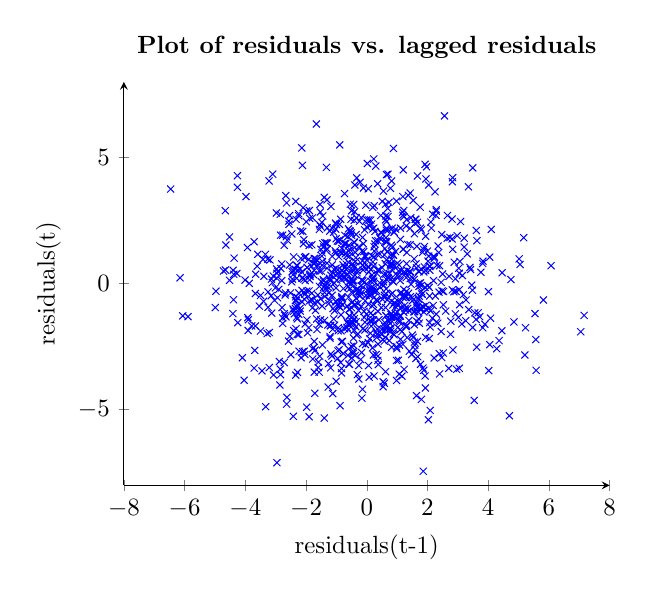
\begin{tikzpicture}[scale=0.9]
	\begin{axis}[
	xmin=-8, xmax=8, xlabel=residuals(t-1),
	ymin=-8, ymax=8, ylabel=residuals(t),
	samples=400,
	axis x line=bottom,
	axis y line=left,
	domain=-8:-8,
	title=\textbf{Plot of residuals vs. lagged residuals}
	]
	\addplot[mark=x,blue, only marks] coordinates {
		(3.67,-1.16)
		(-4.52,1.85)
		(1.72,0.01)
		(0.64,-1.27)
		(-2.62,1.72)
		(-0.87,-0.96)
		(0.69,2.98)
		(7.16,-1.26)
		(5.54,-1.19)
		(-2.70,-1.26)
		(6.07,0.71)
		(1.45,2.61)
		(-0.13,0.73)
		(1.43,1.54)
		(-0.41,2.51)
		(-0.25,-0.26)
		(2.98,1.90)
		(2.82,-0.25)
		(2.83,4.20)
		(1.34,0.52)
		(-2.41,-1.09)
		(1.43,0.20)
		(3.26,-1.47)
		(0.98,-3.05)
		(2.07,0.70)
		(1.45,0.47)
		(-0.61,1.31)
		(0.59,-1.69)
		(-1.57,-1.61)
		(1.78,-0.98)
		(-2.29,-2.01)
		(-2.14,5.38)
		(-1.62,0.74)
		(-5.89,-1.31)
		(2.88,0.85)
		(0.65,2.46)
		(-1.51,1.36)
		(2.74,1.83)
		(-3.42,0.96)
		(-0.20,-3.01)
		(-0.48,-1.52)
		(0.64,2.12)
		(0.63,-0.40)
		(-1.73,0.52)
		(-0.06,1.11)
		(-0.33,-2.04)
		(1.26,0.38)
		(2.19,-0.87)
		(2.22,-2.95)
		(-1.73,0.79)
		(0.15,-1.69)
		(-2.43,-1.01)
		(-2.23,-2.68)
		(-0.01,-1.21)
		(3.07,0.88)
		(-1.54,3.14)
		(0.74,-2.26)
		(-0.45,0.69)
		(2.23,1.05)
		(-2.18,2.09)
		(0.07,2.52)
		(1.11,-2.21)
		(2.20,0.12)
		(3.09,2.46)
		(0.17,1.09)
		(-2.98,2.80)
		(-1.48,2.43)
		(-2.12,4.69)
		(4.70,-5.24)
		(-1.23,-0.66)
		(1.50,-0.68)
		(-0.38,-2.85)
		(1.78,-1.04)
		(-1.53,2.84)
		(-2.80,0.12)
		(-2.84,1.92)
		(0.98,3.27)
		(-0.35,-0.58)
		(-0.39,-0.82)
		(2.84,-2.63)
		(0.58,-0.55)
		(0.40,-1.43)
		(3.18,-0.44)
		(-1.61,-0.45)
		(1.39,-1.46)
		(1.67,-2.29)
		(-0.49,-0.76)
		(0.43,0.03)
		(-2.33,-1.79)
		(-2.30,0.70)
		(0.21,-0.29)
		(1.44,-0.52)
		(5.17,1.82)
		(-1.33,4.61)
		(0.37,1.70)
		(-0.16,1.29)
		(-3.87,0.01)
		(-0.88,0.26)
		(-3.59,1.16)
		(1.68,-1.11)
		(-1.78,-2.99)
		(0.20,0.86)
		(-1.09,-1.40)
		(0.61,0.79)
		(-1.20,-1.66)
		(0.98,-2.51)
		(1.48,-2.81)
		(3.42,0.56)
		(-0.39,3.91)
		(-4.28,0.40)
		(-1.68,0.98)
		(2.71,0.29)
		(-2.14,0.46)
		(1.92,4.73)
		(0.25,-1.56)
		(2.87,-0.32)
		(-3.92,-1.35)
		(-0.40,1.43)
		(-2.42,0.51)
		(5.82,-0.65)
		(1.65,1.48)
		(2.76,-2.01)
		(-2.12,0.24)
		(-0.94,0.40)
		(-0.54,3.15)
		(2.20,1.08)
		(-0.56,0.07)
		(1.40,-2.68)
		(-4.10,-2.94)
		(-0.71,1.18)
		(-1.65,-1.40)
		(-3.15,-0.48)
		(1.02,-1.74)
		(0.56,0.36)
		(0.07,0.46)
		(-2.67,3.49)
		(2.25,3.64)
		(0.70,2.12)
		(-0.60,2.17)
		(0.05,-2.34)
		(-0.52,2.55)
		(-3.50,-1.88)
		(-0.57,-3.20)
		(-1.66,6.33)
		(-1.96,0.64)
		(-2.31,-1.33)
		(-1.07,0.02)
		(-4.01,0.14)
		(1.93,-4.14)
		(1.04,-1.43)
		(-0.04,1.06)
		(-0.07,0.07)
		(-1.60,-3.33)
		(2.04,-0.98)
		(-0.27,-0.30)
		(-1.43,0.16)
		(2.70,-3.36)
		(-0.45,0.51)
		(-1.18,3.06)
		(-0.59,-3.19)
		(-1.70,0.88)
		(-2.24,2.69)
		(5.05,0.76)
		(3.31,1.18)
		(0.62,-0.95)
		(-2.51,-0.37)
		(-1.73,-2.29)
		(-0.35,-0.24)
		(1.58,-1.11)
		(-2.66,-1.32)
		(-4.66,2.89)
		(-2.90,-0.23)
		(0.67,1.26)
		(0.78,0.75)
		(0.90,-2.03)
		(-0.26,-3.78)
		(0.37,-2.87)
		(-0.95,0.55)
		(1.72,-0.60)
		(-2.72,1.52)
		(0.91,-0.76)
		(-1.70,-2.64)
		(-0.67,0.19)
		(1.11,2.20)
		(2.08,0.53)
		(-2.24,-0.37)
		(2.52,-0.84)
		(1.32,2.54)
		(-0.14,1.83)
		(-0.39,-0.86)
		(-0.44,-2.69)
		(-0.61,-1.83)
		(0.05,0.67)
		(0.10,-2.19)
		(1.65,-0.77)
		(3.05,-0.24)
		(0.93,-1.32)
		(-0.42,-1.25)
		(1.25,-0.45)
		(0.37,-1.10)
		(-2.06,-2.68)
		(1.90,1.47)
		(0.61,-1.84)
		(0.27,2.07)
		(1.03,-0.69)
		(0.52,-0.62)
		(-1.88,2.59)
		(-0.32,0.52)
		(-0.29,-0.80)
		(-1.06,-1.65)
		(3.36,-1.03)
		(-1.75,0.80)
		(-0.97,1.69)
		(-1.42,0.10)
		(-2.35,-0.99)
		(-0.38,0.67)
		(-0.55,1.34)
		(3.06,-0.84)
		(-0.50,2.89)
		(-2.13,-0.73)
		(3.21,1.80)
		(2.47,1.94)
		(-0.46,0.11)
		(-3.01,-0.17)
		(-0.89,1.74)
		(-0.31,-3.61)
		(0.55,0.07)
		(-0.52,0.14)
		(0.89,0.73)
		(0.78,-1.77)
		(-2.50,-2.82)
		(-1.90,-5.28)
		(-1.48,1.09)
		(-1.02,2.16)
		(-0.64,-0.89)
		(0.02,4.76)
		(-6.06,-1.28)
		(-0.91,-2.62)
		(2.48,-0.29)
		(-2.13,0.21)
		(1.87,1.36)
		(0.70,0.24)
		(-0.06,-1.53)
		(0.36,-3.05)
		(-3.13,-1.17)
		(-0.17,-2.73)
		(3.21,1.45)
		(0.20,-0.21)
		(0.08,-3.71)
		(-1.47,0.73)
		(-0.06,-1.84)
		(0.46,2.70)
		(0.85,0.10)
		(-0.75,0.46)
		(-0.47,-1.57)
		(4.05,1.05)
		(-4.52,0.13)
		(4.46,0.43)
		(0.68,-0.64)
		(2.00,1.29)
		(-3.33,-4.88)
		(-1.18,0.33)
		(-0.56,2.10)
		(0.85,-0.38)
		(-3.34,1.16)
		(0.94,-1.19)
		(-2.43,0.35)
		(0.13,-1.17)
		(1.30,2.29)
		(0.65,0.94)
		(2.17,2.75)
		(2.01,-0.08)
		(-1.30,-0.12)
		(0.51,0.63)
		(-1.89,2.90)
		(-2.64,-4.78)
		(1.85,-3.35)
		(0.00,2.53)
		(-0.11,3.79)
		(1.82,-0.41)
		(1.19,2.71)
		(0.70,4.34)
		(2.50,0.38)
		(1.86,-0.91)
		(0.48,-0.95)
		(-1.38,-0.51)
		(-1.30,1.60)
		(2.38,-0.34)
		(-3.22,4.07)
		(-0.05,-0.68)
		(-3.90,-1.43)
		(2.04,1.09)
		(1.72,0.47)
		(0.00,0.93)
		(-0.14,-4.19)
		(-4.97,-0.30)
		(1.16,-3.67)
		(-4.38,0.37)
		(-4.64,1.53)
		(0.16,2.36)
		(-1.90,1.51)
		(0.82,0.97)
		(1.35,1.55)
		(1.72,-0.11)
		(-1.38,-0.08)
		(0.90,2.04)
		(0.20,2.17)
		(1.65,-0.94)
		(1.07,-3.59)
		(1.80,-4.59)
		(-0.26,-3.25)
		(-0.29,-2.00)
		(2.02,0.89)
		(-4.25,-1.55)
		(-1.01,-0.17)
		(-2.54,0.74)
		(-0.77,-2.77)
		(1.30,-1.70)
		(1.65,-1.50)
		(-2.03,-1.60)
		(-0.94,-0.88)
		(0.27,1.57)
		(-0.58,-1.01)
		(0.60,1.39)
		(0.80,0.68)
		(-1.86,0.38)
		(-0.35,1.95)
		(-4.26,4.28)
		(2.29,2.93)
		(-1.26,-3.17)
		(-2.41,1.06)
		(-0.51,-2.49)
		(-2.86,-4.02)
		(-0.04,-2.42)
		(-1.12,-4.36)
		(4.36,-2.26)
		(2.28,2.71)
		(-4.99,-0.95)
		(0.88,5.36)
		(-2.80,0.78)
		(-0.51,2.01)
		(0.33,-0.29)
		(1.50,-0.56)
		(-0.55,-1.57)
		(3.15,0.32)
		(-0.96,-2.97)
		(0.66,-1.70)
		(1.33,-2.14)
		(0.17,0.34)
		(1.76,3.03)
		(0.65,4.32)
		(-1.57,-3.51)
		(-3.61,0.69)
		(3.72,-1.31)
		(-1.21,-2.16)
		(0.21,0.21)
		(1.13,-0.94)
		(0.23,0.10)
		(-1.81,1.54)
		(-0.94,-1.87)
		(-0.25,-0.31)
		(2.96,-3.40)
		(-1.72,-0.77)
		(1.57,1.98)
		(0.62,-3.49)
		(-0.47,0.78)
		(-2.11,-2.70)
		(-0.57,0.44)
		(-0.17,-0.90)
		(-2.94,-0.56)
		(0.38,-3.21)
		(-1.64,-1.82)
		(-0.19,-0.39)
		(0.67,0.14)
		(-1.81,-0.38)
		(-0.58,-1.28)
		(0.70,2.66)
		(-3.67,-0.39)
		(2.07,-1.55)
		(4.85,-1.52)
		(1.92,-0.15)
		(-0.63,1.86)
		(0.86,-0.85)
		(-2.07,1.74)
		(3.76,0.45)
		(1.88,-1.13)
		(1.57,-1.63)
		(-1.75,0.35)
		(0.64,-0.21)
		(-1.12,-1.81)
		(-0.62,-1.59)
		(-1.14,1.08)
		(-2.05,1.04)
		(-1.82,-0.62)
		(-0.42,1.65)
		(-3.40,-0.70)
		(1.22,-0.23)
		(-0.24,2.47)
		(1.40,-1.08)
		(0.54,-4.09)
		(0.99,-2.58)
		(-2.97,0.58)
		(-2.04,-0.43)
		(-0.89,5.50)
		(0.22,-2.83)
		(2.26,-0.49)
		(-0.58,0.08)
		(2.52,-2.75)
		(0.95,2.16)
		(2.35,1.49)
		(0.25,3.09)
		(-1.31,1.38)
		(-2.96,-7.10)
		(0.31,-1.93)
		(1.64,0.62)
		(-0.59,-1.63)
		(-1.08,0.57)
		(-0.62,-0.13)
		(-2.19,-1.09)
		(-0.99,0.14)
		(-0.36,1.03)
		(0.09,2.29)
		(-0.13,-1.79)
		(1.22,-1.14)
		(0.22,-1.44)
		(3.63,1.70)
		(0.62,3.15)
		(3.61,2.11)
		(-1.45,2.68)
		(1.05,0.50)
		(-0.52,-1.60)
		(1.20,1.36)
		(1.19,3.45)
		(-4.37,1.01)
		(-2.65,1.86)
		(-2.88,-3.09)
		(0.80,1.14)
		(2.94,-0.31)
		(-0.65,1.11)
		(1.62,2.55)
		(1.09,-1.28)
		(-2.10,3.01)
		(0.79,-1.89)
		(-1.50,0.08)
		(3.03,0.61)
		(-0.07,2.13)
		(3.27,-0.65)
		(-0.85,-1.87)
		(1.18,2.83)
		(-0.13,0.73)
		(-4.04,-3.83)
		(-1.96,0.64)
		(1.23,-3.40)
		(-0.11,1.58)
		(-2.24,2.77)
		(-1.25,-0.37)
		(0.50,-1.82)
		(-1.99,2.45)
		(1.95,-1.02)
		(-1.28,-1.64)
		(3.62,-2.52)
		(-2.16,-2.94)
		(0.40,0.55)
		(-3.04,-0.66)
		(-1.45,1.58)
		(-1.19,-0.11)
		(0.80,-0.42)
		(1.88,-3.44)
		(0.60,-1.55)
		(-0.75,0.21)
		(1.63,-0.86)
		(1.60,2.55)
		(0.24,-3.66)
		(1.14,-0.36)
		(0.83,0.23)
		(-1.97,-1.44)
		(1.52,0.22)
		(-1.31,3.32)
		(-1.21,-2.10)
		(0.35,-0.70)
		(-0.62,-2.84)
		(-0.26,1.46)
		(1.19,-2.41)
		(2.09,-1.72)
		(-0.40,2.85)
		(0.66,1.65)
		(-0.48,-1.51)
		(0.46,2.03)
		(0.88,-1.32)
		(-1.23,0.21)
		(0.55,3.67)
		(1.20,4.51)
		(0.18,-0.89)
		(3.46,-0.06)
		(-1.22,2.08)
		(-1.47,1.22)
		(-3.50,-0.47)
		(1.82,-0.42)
		(1.73,-1.57)
		(-0.16,-4.54)
		(1.80,-0.31)
		(0.37,-2.40)
		(0.58,-0.46)
		(0.23,4.94)
		(0.88,0.07)
		(0.20,3.02)
		(5.57,-2.22)
		(-2.33,2.55)
		(-3.71,-3.35)
		(-2.28,-0.56)
		(-2.19,0.58)
		(-0.87,1.24)
		(-0.34,-0.25)
		(-0.44,-2.16)
		(1.08,-2.44)
		(0.78,-1.44)
		(1.50,-2.04)
		(3.56,-1.16)
		(2.45,-1.90)
		(-2.57,2.48)
		(-4.66,0.54)
		(1.80,0.57)
		(-3.67,-1.68)
		(0.13,0.55)
		(0.07,0.65)
		(4.45,-1.87)
		(-0.14,-2.38)
		(-1.01,-3.87)
		(0.47,1.75)
		(0.49,-2.02)
		(0.14,0.09)
		(-1.22,0.17)
		(-2.45,0.18)
		(0.63,-1.28)
		(-2.69,-0.45)
		(-2.06,-0.61)
		(2.66,2.70)
		(-0.84,-2.31)
		(-0.28,-0.41)
		(1.80,2.13)
		(-0.60,0.84)
		(2.06,-2.18)
		(-0.69,1.59)
		(2.03,-5.40)
		(1.26,-0.99)
		(-0.43,3.14)
		(-1.73,1.00)
		(-2.09,1.58)
		(-0.54,-0.19)
		(-0.88,-0.76)
		(-0.82,1.39)
		(1.97,4.63)
		(-0.60,-0.54)
		(2.29,2.87)
		(-1.06,-1.08)
		(1.95,-0.86)
		(-1.04,1.30)
		(0.35,-1.80)
		(1.94,1.88)
		(-0.83,-3.37)
		(-0.88,-4.84)
		(4.01,-0.32)
		(1.90,0.66)
		(-0.86,2.55)
		(1.30,0.24)
		(-0.72,1.91)
		(1.41,0.48)
		(2.83,1.36)
		(-3.21,-1.94)
		(2.06,-0.15)
		(2.92,-1.20)
		(0.09,-0.47)
		(3.49,4.59)
		(0.31,-2.81)
		(-2.47,0.07)
		(-4.39,-0.64)
		(-0.67,0.76)
		(1.43,3.59)
		(0.63,1.82)
		(0.83,-1.31)
		(-1.15,-2.87)
		(0.29,1.70)
		(-3.28,-1.98)
		(-1.52,-1.43)
		(-1.64,0.93)
		(1.04,-3.04)
		(-0.03,3.11)
		(-2.31,0.21)
		(-0.02,-0.47)
		(-1.38,1.62)
		(-1.33,1.61)
		(1.73,-0.50)
		(0.23,2.20)
		(0.80,0.73)
		(1.77,2.20)
		(0.36,0.53)
		(1.10,-0.38)
		(1.37,3.50)
		(2.34,-1.57)
		(0.95,1.27)
		(2.82,4.04)
		(0.05,-0.83)
		(-0.10,1.27)
		(3.40,0.64)
		(-1.02,-0.70)
		(-0.01,-0.01)
		(1.84,1.24)
		(0.30,4.66)
		(2.81,1.77)
		(2.07,-0.49)
		(0.58,-3.95)
		(-1.56,0.50)
		(1.13,0.52)
		(-2.77,-1.58)
		(0.49,2.02)
		(1.62,0.78)
		(0.43,1.17)
		(1.76,-0.97)
		(4.08,-1.37)
		(1.85,-0.93)
		(0.53,-2.22)
		(1.28,-1.05)
		(0.85,1.45)
		(-2.63,-4.51)
		(-0.83,-3.54)
		(2.45,0.05)
		(-0.09,0.66)
		(1.16,-1.90)
		(-2.01,1.07)
		(0.13,2.52)
		(1.20,1.37)
		(-2.72,-3.13)
		(0.70,-1.46)
		(-0.36,-1.71)
		(-1.88,-0.68)
		(-0.08,-1.34)
		(-3.79,-1.68)
		(-4.26,3.82)
		(-2.35,-0.67)
		(-1.98,-0.30)
		(-2.35,0.57)
		(-3.45,-3.46)
		(0.58,-2.28)
		(-3.19,0.94)
		(0.22,0.70)
		(1.57,-2.32)
		(-0.00,2.25)
		(0.19,-0.13)
		(-0.76,0.28)
		(-2.97,0.22)
		(-0.09,-1.10)
		(1.92,-3.66)
		(3.48,-0.26)
		(-0.86,-3.13)
		(-3.25,-0.33)
		(0.33,0.41)
		(0.75,0.40)
		(-0.45,-2.77)
		(-2.30,0.73)
		(4.05,-2.42)
		(-4.72,0.50)
		(-1.02,1.21)
		(-2.64,3.20)
		(-1.27,-4.10)
		(0.64,1.66)
		(0.28,-0.32)
		(-1.42,-0.15)
		(1.55,-1.12)
		(1.24,0.47)
		(1.29,-0.52)
		(-0.85,-1.24)
		(2.10,-1.08)
		(1.32,1.23)
		(5.02,0.98)
		(2.13,2.20)
		(2.31,0.73)
		(0.11,-0.29)
		(-2.58,-2.28)
		(-0.74,0.63)
		(-1.52,-0.61)
		(-1.13,0.44)
		(1.11,1.75)
		(-1.11,-0.99)
		(-1.79,-0.96)
		(-0.82,-0.52)
		(-0.32,0.43)
		(0.82,4.07)
		(-1.91,-1.75)
		(0.63,2.68)
		(0.16,-0.43)
		(2.65,1.80)
		(-0.43,0.12)
		(-0.27,-1.07)
		(-2.34,-0.52)
		(-2.77,1.92)
		(0.62,2.53)
		(-0.50,1.92)
		(1.01,-1.13)
		(-1.79,-2.58)
		(3.82,0.80)
		(0.24,1.06)
		(2.09,-5.03)
		(-0.45,0.05)
		(-0.33,4.19)
		(1.38,-0.38)
		(1.11,-1.29)
		(-2.24,-2.02)
		(-3.07,-3.62)
		(-2.20,-0.98)
		(-2.83,0.60)
		(0.12,-1.97)
		(-0.82,0.51)
		(-0.74,1.58)
		(-2.72,-1.19)
		(1.56,0.98)
		(0.88,1.13)
		(-0.18,-0.09)
		(2.04,3.91)
		(-1.75,-2.54)
		(0.83,0.55)
		(0.70,-1.85)
		(0.70,-1.44)
		(-1.46,0.88)
		(0.65,2.19)
		(-1.03,0.34)
		(-1.79,2.61)
		(-2.41,-1.86)
		(2.08,0.68)
		(-1.69,-1.06)
		(-0.35,-1.51)
		(-2.42,-5.26)
		(-0.59,1.52)
		(-6.46,3.75)
		(-2.17,1.00)
		(-2.85,2.75)
		(-2.03,0.12)
		(-0.43,-2.46)
		(-0.65,-1.74)
		(3.89,-1.61)
		(-1.14,2.20)
		(-0.50,-0.96)
		(-3.14,0.18)
		(-0.95,-2.67)
		(-2.68,-0.37)
		(0.06,-3.25)
		(1.71,-1.40)
		(0.81,1.52)
		(-1.40,3.42)
		(-3.26,0.97)
		(2.92,0.19)
		(4.10,2.15)
		(0.24,1.46)
		(-1.98,-4.90)
		(2.40,-3.58)
		(-1.19,-1.67)
		(-0.94,-1.75)
		(1.77,-3.20)
		(-2.77,-1.36)
		(-3.91,-1.86)
		(0.84,2.20)
		(0.80,-1.22)
		(0.19,-2.55)
		(0.99,-0.83)
		(2.16,-1.37)
		(1.94,0.52)
		(-1.14,-0.46)
		(1.62,-2.97)
		(0.35,1.16)
		(-1.01,-0.73)
		(-2.39,-1.20)
		(1.29,-1.70)
		(-0.71,1.59)
		(0.09,-0.22)
		(-1.59,-3.11)
		(-3.10,4.34)
		(0.34,-0.68)
		(-0.12,0.54)
		(2.40,0.71)
		(1.60,-2.61)
		(2.11,2.44)
		(-1.50,0.50)
		(-1.87,0.29)
		(-2.54,2.70)
		(1.00,0.32)
		(5.58,-3.44)
		(1.46,-0.03)
		(-1.55,2.33)
		(1.67,2.43)
		(-2.26,0.53)
		(-2.85,-3.39)
		(1.43,2.19)
		(-1.56,-0.11)
		(0.63,0.38)
		(2.81,2.56)
		(0.80,0.81)
		(1.86,-7.44)
		(-3.21,-3.33)
		(1.32,-1.66)
		(4.28,-2.58)
		(1.08,0.31)
		(-3.08,0.30)
		(-0.41,-1.39)
		(-1.00,2.34)
		(0.77,-1.58)
		(0.82,-0.69)
		(0.81,-1.33)
		(-0.73,-1.79)
		(-1.20,0.11)
		(-1.18,-2.79)
		(1.71,-0.62)
		(-3.71,1.66)
		(-0.41,1.63)
		(0.54,-3.89)
		(-1.31,0.81)
		(0.95,-0.92)
		(-0.14,0.90)
		(-1.88,0.34)
		(0.32,-0.63)
		(-0.54,-0.03)
		(-0.82,1.22)
		(-1.42,1.45)
		(0.12,-1.50)
		(-3.69,-2.65)
		(-0.80,-0.84)
		(-1.09,2.04)
		(-1.82,0.69)
		(1.31,0.79)
		(-1.47,-0.89)
		(1.08,-1.53)
		(1.95,4.15)
		(-0.31,-0.21)
		(0.56,-0.07)
		(1.28,-0.55)
		(-0.16,0.14)
		(1.08,-0.64)
		(-2.53,-2.09)
		(2.22,0.99)
		(-1.98,2.88)
		(-3.66,0.37)
		(2.77,-1.49)
		(-0.13,0.11)
		(0.90,2.04)
		(-0.73,3.57)
		(-2.04,-2.81)
		(-6.15,0.23)
		(1.25,-0.87)
		(-0.57,1.09)
		(-0.39,0.34)
		(0.81,-1.18)
		(-2.84,-3.61)
		(-1.46,-2.43)
		(2.29,-1.21)
		(1.20,-0.55)
		(-2.56,2.35)
		(-4.41,-1.19)
		(-1.14,0.74)
		(0.43,1.81)
		(1.88,0.46)
		(0.19,0.17)
		(-2.24,-1.22)
		(0.61,1.68)
		(-2.34,3.26)
		(-1.92,0.95)
		(-1.31,0.61)
		(-2.46,0.47)
		(-0.54,2.07)
		(-1.80,-0.66)
		(-0.57,-1.02)
		(-0.92,1.06)
		(-0.82,-0.61)
		(-1.01,1.78)
		(2.47,-2.93)
		(1.22,2.65)
		(0.12,-1.46)
		(-2.93,0.48)
		(-3.25,-0.94)
		(-3.93,1.43)
		(5.21,-2.83)
		(1.94,-2.13)
		(0.51,3.26)
		(-1.95,-1.95)
		(-2.29,-1.40)
		(1.10,0.12)
		(3.13,-1.60)
		(-3.39,0.29)
		(-0.90,2.35)
		(-0.17,0.14)
		(-3.98,3.45)
		(1.68,-2.90)
		(-0.83,-0.57)
		(3.82,-1.75)
		(-0.78,0.74)
		(0.82,-2.52)
		(-2.28,-3.52)
		(-1.25,-0.79)
		(-2.34,-3.63)
		(0.79,-1.80)
		(2.60,-1.09)
		(-1.19,-3.34)
		(0.87,1.13)
		(-1.01,0.61)
		(0.20,-1.25)
		(2.39,-2.78)
		(0.24,-0.55)
		(-2.07,-0.34)
		(-1.71,-4.35)
		(-0.34,2.61)
		(-0.38,0.87)
		(-1.73,-3.51)
		(0.36,3.96)
		(2.53,-0.31)
		(-0.50,-2.95)
		(-0.41,-1.85)
		(-4.40,0.53)
		(-1.55,-2.88)
		(-2.79,-0.95)
		(-0.77,-0.20)
		(1.05,-0.85)
		(3.05,0.41)
		(3.60,-1.42)
		(-0.23,-0.50)
		(-0.64,0.38)
		(1.64,-4.44)
		(0.98,-3.84)
		(1.53,-2.13)
		(1.56,0.16)
		(-2.96,0.41)
		(1.08,-1.46)
		(-0.18,2.62)
		(-1.52,2.27)
		(-1.39,-0.35)
		(2.56,6.65)
		(-1.62,-0.73)
		(-2.47,1.97)
		(0.43,-0.13)
		(4.02,-3.45)
		(0.05,3.76)
		(0.62,-2.13)
		(-1.88,0.15)
		(3.35,3.84)
		(0.25,1.29)
		(1.06,0.74)
		(-1.90,-0.29)
		(1.71,0.49)
		(0.78,3.78)
		(-2.31,-0.92)
		(0.08,-0.44)
		(-0.90,-0.91)
		(0.22,-0.82)
		(-0.50,-0.34)
		(-0.38,1.24)
		(-2.07,0.18)
		(-0.65,-1.52)
		(1.53,3.30)
		(3.49,-1.74)
		(-2.32,-0.66)
		(4.75,0.16)
		(3.05,-3.36)
		(0.34,-2.02)
		(-0.60,-2.59)
		(-1.40,-5.33)
		(1.67,4.27)
		(-1.39,-1.46)
		(-0.92,1.68)
		(1.77,0.03)
		(0.87,-1.99)
		(1.79,-0.08)
		(1.01,0.81)
		(-0.80,-2.29)
		(-1.03,2.40)
		(1.59,2.39)
		(-1.34,-0.19)
		(2.37,1.23)
		(1.58,-2.44)
		(0.58,1.14)
		(0.01,-0.26)
		(0.73,3.22)
		(7.05,-1.91)
		(-0.22,4.02)
		(-3.11,0.04)
		(3.83,0.89)
		(1.22,2.90)
		(-1.30,2.21)
		(5.23,-1.75)
		(1.10,-1.83)
		(0.59,-1.83)
		(-1.56,2.15)
		(-2.13,-0.27)
		(-3.54,-0.89)
		(-0.85,0.17)
		(-2.11,2.07)
		(1.30,-0.32)
		(-0.64,0.62)
		(3.54,-4.63)
		(3.02,-1.34)
		(0.33,-2.13)
		(-0.57,-1.28)
		(2.30,-1.52)
		(-2.29,-0.84)
		(1.35,-0.98)
		(-1.34,1.32)
	};
	\end{axis}
	\end{tikzpicture}
	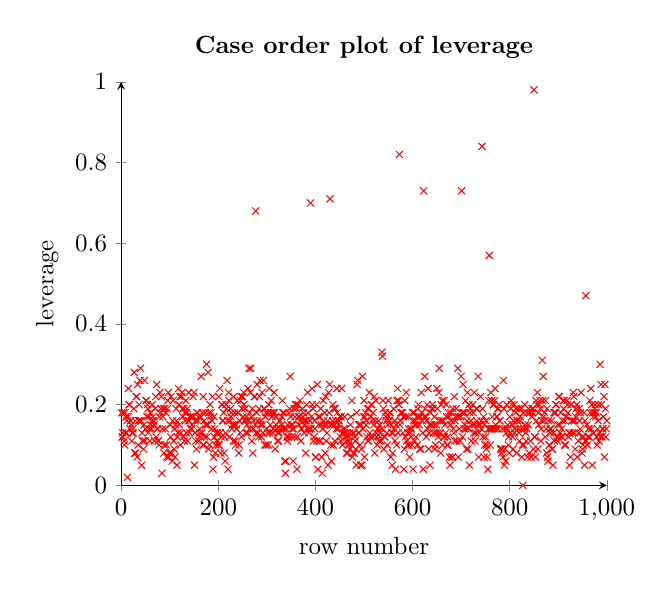
\begin{tikzpicture}[scale=0.9]
	\begin{axis}[
	xmin=0, xmax=1000, xlabel=row number,
	ymin=0, ymax=1, ylabel=leverage,
	axis x line=bottom,
	axis y line=left,
	title=\textbf{Case order plot of leverage}
	]
	\addplot[mark=x,red, only marks] coordinates {
		(1.00,0.18)
		(2.00,0.12)
		(3.00,0.13)
		(4.00,0.12)
		(5.00,0.18)
		(6.00,0.11)
		(7.00,0.10)
		(8.00,0.18)
		(9.00,0.13)
		(10.00,0.17)
		(11.00,0.13)
		(12.00,0.16)
		(13.00,0.02)
		(14.00,0.17)
		(15.00,0.24)
		(16.00,0.20)
		(17.00,0.20)
		(18.00,0.14)
		(19.00,0.16)
		(20.00,0.16)
		(21.00,0.15)
		(22.00,0.11)
		(23.00,0.13)
		(24.00,0.14)
		(25.00,0.13)
		(26.00,0.19)
		(27.00,0.28)
		(28.00,0.08)
		(29.00,0.16)
		(30.00,0.08)
		(31.00,0.22)
		(32.00,0.22)
		(33.00,0.07)
		(34.00,0.25)
		(35.00,0.10)
		(36.00,0.16)
		(37.00,0.20)
		(38.00,0.16)
		(39.00,0.26)
		(40.00,0.29)
		(41.00,0.16)
		(42.00,0.05)
		(43.00,0.13)
		(44.00,0.11)
		(45.00,0.11)
		(46.00,0.09)
		(47.00,0.15)
		(48.00,0.26)
		(49.00,0.11)
		(50.00,0.14)
		(51.00,0.21)
		(52.00,0.21)
		(53.00,0.17)
		(54.00,0.20)
		(55.00,0.19)
		(56.00,0.13)
		(57.00,0.17)
		(58.00,0.14)
		(59.00,0.11)
		(60.00,0.18)
		(61.00,0.15)
		(62.00,0.14)
		(63.00,0.16)
		(64.00,0.20)
		(65.00,0.17)
		(66.00,0.16)
		(67.00,0.16)
		(68.00,0.15)
		(69.00,0.11)
		(70.00,0.19)
		(71.00,0.22)
		(72.00,0.12)
		(73.00,0.25)
		(74.00,0.14)
		(75.00,0.14)
		(76.00,0.11)
		(77.00,0.11)
		(78.00,0.10)
		(79.00,0.17)
		(80.00,0.23)
		(81.00,0.18)
		(82.00,0.19)
		(83.00,0.22)
		(84.00,0.03)
		(85.00,0.14)
		(86.00,0.17)
		(87.00,0.19)
		(88.00,0.08)
		(89.00,0.10)
		(90.00,0.19)
		(91.00,0.14)
		(92.00,0.18)
		(93.00,0.10)
		(94.00,0.07)
		(95.00,0.19)
		(96.00,0.21)
		(97.00,0.23)
		(98.00,0.07)
		(99.00,0.08)
		(100.00,0.08)
		(101.00,0.15)
		(102.00,0.12)
		(103.00,0.22)
		(104.00,0.08)
		(105.00,0.06)
		(106.00,0.16)
		(107.00,0.21)
		(108.00,0.11)
		(109.00,0.09)
		(110.00,0.14)
		(111.00,0.07)
		(112.00,0.15)
		(113.00,0.19)
		(114.00,0.16)
		(115.00,0.05)
		(116.00,0.12)
		(117.00,0.13)
		(118.00,0.24)
		(119.00,0.20)
		(120.00,0.15)
		(121.00,0.22)
		(122.00,0.10)
		(123.00,0.13)
		(124.00,0.22)
		(125.00,0.23)
		(126.00,0.19)
		(127.00,0.17)
		(128.00,0.12)
		(129.00,0.19)
		(130.00,0.11)
		(131.00,0.18)
		(132.00,0.16)
		(133.00,0.21)
		(134.00,0.13)
		(135.00,0.18)
		(136.00,0.19)
		(137.00,0.11)
		(138.00,0.16)
		(139.00,0.23)
		(140.00,0.16)
		(141.00,0.13)
		(142.00,0.17)
		(143.00,0.14)
		(144.00,0.17)
		(145.00,0.14)
		(146.00,0.15)
		(147.00,0.17)
		(148.00,0.22)
		(149.00,0.17)
		(150.00,0.23)
		(151.00,0.05)
		(152.00,0.13)
		(153.00,0.16)
		(154.00,0.11)
		(155.00,0.09)
		(156.00,0.18)
		(157.00,0.18)
		(158.00,0.16)
		(159.00,0.17)
		(160.00,0.11)
		(161.00,0.13)
		(162.00,0.14)
		(163.00,0.12)
		(164.00,0.17)
		(165.00,0.27)
		(166.00,0.13)
		(167.00,0.18)
		(168.00,0.10)
		(169.00,0.22)
		(170.00,0.10)
		(171.00,0.16)
		(172.00,0.12)
		(173.00,0.18)
		(174.00,0.15)
		(175.00,0.15)
		(176.00,0.30)
		(177.00,0.12)
		(178.00,0.15)
		(179.00,0.28)
		(180.00,0.09)
		(181.00,0.18)
		(182.00,0.10)
		(183.00,0.20)
		(184.00,0.17)
		(185.00,0.18)
		(186.00,0.14)
		(187.00,0.16)
		(188.00,0.22)
		(189.00,0.04)
		(190.00,0.07)
		(191.00,0.17)
		(192.00,0.12)
		(193.00,0.14)
		(194.00,0.08)
		(195.00,0.10)
		(196.00,0.13)
		(197.00,0.11)
		(198.00,0.11)
		(199.00,0.13)
		(200.00,0.10)
		(201.00,0.22)
		(202.00,0.10)
		(203.00,0.24)
		(204.00,0.13)
		(205.00,0.08)
		(206.00,0.12)
		(207.00,0.20)
		(208.00,0.20)
		(209.00,0.16)
		(210.00,0.16)
		(211.00,0.18)
		(212.00,0.08)
		(213.00,0.12)
		(214.00,0.06)
		(215.00,0.13)
		(216.00,0.20)
		(217.00,0.19)
		(218.00,0.26)
		(219.00,0.16)
		(220.00,0.04)
		(221.00,0.23)
		(222.00,0.21)
		(223.00,0.12)
		(224.00,0.16)
		(225.00,0.19)
		(226.00,0.17)
		(227.00,0.18)
		(228.00,0.14)
		(229.00,0.15)
		(230.00,0.15)
		(231.00,0.11)
		(232.00,0.22)
		(233.00,0.15)
		(234.00,0.18)
		(235.00,0.11)
		(236.00,0.10)
		(237.00,0.15)
		(238.00,0.14)
		(239.00,0.21)
		(240.00,0.18)
		(241.00,0.18)
		(242.00,0.08)
		(243.00,0.10)
		(244.00,0.16)
		(245.00,0.13)
		(246.00,0.21)
		(247.00,0.22)
		(248.00,0.12)
		(249.00,0.19)
		(250.00,0.22)
		(251.00,0.17)
		(252.00,0.23)
		(253.00,0.20)
		(254.00,0.16)
		(255.00,0.19)
		(256.00,0.16)
		(257.00,0.13)
		(258.00,0.17)
		(259.00,0.15)
		(260.00,0.13)
		(261.00,0.24)
		(262.00,0.16)
		(263.00,0.29)
		(264.00,0.14)
		(265.00,0.18)
		(266.00,0.23)
		(267.00,0.29)
		(268.00,0.17)
		(269.00,0.11)
		(270.00,0.19)
		(271.00,0.08)
		(272.00,0.14)
		(273.00,0.16)
		(274.00,0.22)
		(275.00,0.22)
		(276.00,0.15)
		(277.00,0.68)
		(278.00,0.13)
		(279.00,0.18)
		(280.00,0.25)
		(281.00,0.16)
		(282.00,0.13)
		(283.00,0.12)
		(284.00,0.19)
		(285.00,0.22)
		(286.00,0.26)
		(287.00,0.15)
		(288.00,0.16)
		(289.00,0.12)
		(290.00,0.23)
		(291.00,0.15)
		(292.00,0.13)
		(293.00,0.26)
		(294.00,0.19)
		(295.00,0.19)
		(296.00,0.10)
		(297.00,0.17)
		(298.00,0.18)
		(299.00,0.10)
		(300.00,0.14)
		(301.00,0.13)
		(302.00,0.18)
		(303.00,0.10)
		(304.00,0.20)
		(305.00,0.24)
		(306.00,0.13)
		(307.00,0.15)
		(308.00,0.18)
		(309.00,0.21)
		(310.00,0.18)
		(311.00,0.17)
		(312.00,0.13)
		(313.00,0.14)
		(314.00,0.18)
		(315.00,0.23)
		(316.00,0.18)
		(317.00,0.09)
		(318.00,0.17)
		(319.00,0.15)
		(320.00,0.14)
		(321.00,0.14)
		(322.00,0.11)
		(323.00,0.13)
		(324.00,0.11)
		(325.00,0.13)
		(326.00,0.16)
		(327.00,0.16)
		(328.00,0.14)
		(329.00,0.14)
		(330.00,0.15)
		(331.00,0.17)
		(332.00,0.21)
		(333.00,0.18)
		(334.00,0.14)
		(335.00,0.18)
		(336.00,0.14)
		(337.00,0.06)
		(338.00,0.03)
		(339.00,0.06)
		(340.00,0.14)
		(341.00,0.12)
		(342.00,0.11)
		(343.00,0.15)
		(344.00,0.12)
		(345.00,0.12)
		(346.00,0.18)
		(347.00,0.19)
		(348.00,0.27)
		(349.00,0.17)
		(350.00,0.15)
		(351.00,0.12)
		(352.00,0.14)
		(353.00,0.15)
		(354.00,0.06)
		(355.00,0.14)
		(356.00,0.19)
		(357.00,0.12)
		(358.00,0.17)
		(359.00,0.20)
		(360.00,0.20)
		(361.00,0.19)
		(362.00,0.04)
		(363.00,0.12)
		(364.00,0.20)
		(365.00,0.17)
		(366.00,0.15)
		(367.00,0.17)
		(368.00,0.21)
		(369.00,0.16)
		(370.00,0.11)
		(371.00,0.14)
		(372.00,0.14)
		(373.00,0.19)
		(374.00,0.17)
		(375.00,0.18)
		(376.00,0.16)
		(377.00,0.13)
		(378.00,0.15)
		(379.00,0.16)
		(380.00,0.08)
		(381.00,0.16)
		(382.00,0.20)
		(383.00,0.14)
		(384.00,0.23)
		(385.00,0.18)
		(386.00,0.13)
		(387.00,0.14)
		(388.00,0.14)
		(389.00,0.16)
		(390.00,0.70)
		(391.00,0.14)
		(392.00,0.17)
		(393.00,0.24)
		(394.00,0.20)
		(395.00,0.19)
		(396.00,0.11)
		(397.00,0.12)
		(398.00,0.16)
		(399.00,0.14)
		(400.00,0.07)
		(401.00,0.07)
		(402.00,0.20)
		(403.00,0.11)
		(404.00,0.25)
		(405.00,0.04)
		(406.00,0.17)
		(407.00,0.15)
		(408.00,0.11)
		(409.00,0.17)
		(410.00,0.11)
		(411.00,0.19)
		(412.00,0.15)
		(413.00,0.07)
		(414.00,0.03)
		(415.00,0.14)
		(416.00,0.21)
		(417.00,0.16)
		(418.00,0.15)
		(419.00,0.18)
		(420.00,0.08)
		(421.00,0.22)
		(422.00,0.11)
		(423.00,0.15)
		(424.00,0.13)
		(425.00,0.16)
		(426.00,0.05)
		(427.00,0.23)
		(428.00,0.18)
		(429.00,0.25)
		(430.00,0.71)
		(431.00,0.15)
		(432.00,0.10)
		(433.00,0.06)
		(434.00,0.15)
		(435.00,0.16)
		(436.00,0.20)
		(437.00,0.10)
		(438.00,0.19)
		(439.00,0.15)
		(440.00,0.11)
		(441.00,0.19)
		(442.00,0.16)
		(443.00,0.14)
		(444.00,0.24)
		(445.00,0.18)
		(446.00,0.14)
		(447.00,0.16)
		(448.00,0.15)
		(449.00,0.16)
		(450.00,0.17)
		(451.00,0.12)
		(452.00,0.11)
		(453.00,0.17)
		(454.00,0.24)
		(455.00,0.13)
		(456.00,0.10)
		(457.00,0.14)
		(458.00,0.13)
		(459.00,0.13)
		(460.00,0.17)
		(461.00,0.14)
		(462.00,0.12)
		(463.00,0.13)
		(464.00,0.08)
		(465.00,0.11)
		(466.00,0.08)
		(467.00,0.12)
		(468.00,0.10)
		(469.00,0.11)
		(470.00,0.13)
		(471.00,0.09)
		(472.00,0.15)
		(473.00,0.17)
		(474.00,0.10)
		(475.00,0.21)
		(476.00,0.07)
		(477.00,0.13)
		(478.00,0.08)
		(479.00,0.13)
		(480.00,0.08)
		(481.00,0.12)
		(482.00,0.11)
		(483.00,0.09)
		(484.00,0.05)
		(485.00,0.18)
		(486.00,0.25)
		(487.00,0.26)
		(488.00,0.13)
		(489.00,0.15)
		(490.00,0.13)
		(491.00,0.15)
		(492.00,0.10)
		(493.00,0.05)
		(494.00,0.15)
		(495.00,0.09)
		(496.00,0.05)
		(497.00,0.27)
		(498.00,0.14)
		(499.00,0.17)
		(500.00,0.21)
		(501.00,0.07)
		(502.00,0.17)
		(503.00,0.18)
		(504.00,0.15)
		(505.00,0.16)
		(506.00,0.12)
		(507.00,0.19)
		(508.00,0.11)
		(509.00,0.11)
		(510.00,0.19)
		(511.00,0.23)
		(512.00,0.13)
		(513.00,0.12)
		(514.00,0.17)
		(515.00,0.20)
		(516.00,0.20)
		(517.00,0.16)
		(518.00,0.12)
		(519.00,0.18)
		(520.00,0.15)
		(521.00,0.22)
		(522.00,0.08)
		(523.00,0.16)
		(524.00,0.21)
		(525.00,0.13)
		(526.00,0.12)
		(527.00,0.10)
		(528.00,0.14)
		(529.00,0.14)
		(530.00,0.16)
		(531.00,0.11)
		(532.00,0.15)
		(533.00,0.12)
		(534.00,0.13)
		(535.00,0.11)
		(536.00,0.14)
		(537.00,0.33)
		(538.00,0.32)
		(539.00,0.21)
		(540.00,0.19)
		(541.00,0.09)
		(542.00,0.12)
		(543.00,0.12)
		(544.00,0.18)
		(545.00,0.17)
		(546.00,0.16)
		(547.00,0.13)
		(548.00,0.10)
		(549.00,0.15)
		(550.00,0.21)
		(551.00,0.17)
		(552.00,0.16)
		(553.00,0.18)
		(554.00,0.18)
		(555.00,0.07)
		(556.00,0.15)
		(557.00,0.13)
		(558.00,0.05)
		(559.00,0.08)
		(560.00,0.13)
		(561.00,0.19)
		(562.00,0.14)
		(563.00,0.16)
		(564.00,0.11)
		(565.00,0.04)
		(566.00,0.15)
		(567.00,0.10)
		(568.00,0.21)
		(569.00,0.24)
		(570.00,0.13)
		(571.00,0.21)
		(572.00,0.20)
		(573.00,0.82)
		(574.00,0.15)
		(575.00,0.16)
		(576.00,0.18)
		(577.00,0.18)
		(578.00,0.18)
		(579.00,0.18)
		(580.00,0.13)
		(581.00,0.17)
		(582.00,0.04)
		(583.00,0.09)
		(584.00,0.21)
		(585.00,0.12)
		(586.00,0.17)
		(587.00,0.23)
		(588.00,0.11)
		(589.00,0.10)
		(590.00,0.13)
		(591.00,0.17)
		(592.00,0.14)
		(593.00,0.10)
		(594.00,0.07)
		(595.00,0.13)
		(596.00,0.14)
		(597.00,0.12)
		(598.00,0.14)
		(599.00,0.10)
		(600.00,0.18)
		(601.00,0.04)
		(602.00,0.16)
		(603.00,0.18)
		(604.00,0.11)
		(605.00,0.15)
		(606.00,0.16)
		(607.00,0.12)
		(608.00,0.15)
		(609.00,0.17)
		(610.00,0.10)
		(611.00,0.19)
		(612.00,0.20)
		(613.00,0.17)
		(614.00,0.15)
		(615.00,0.09)
		(616.00,0.17)
		(617.00,0.09)
		(618.00,0.23)
		(619.00,0.18)
		(620.00,0.16)
		(621.00,0.13)
		(622.00,0.04)
		(623.00,0.73)
		(624.00,0.17)
		(625.00,0.27)
		(626.00,0.19)
		(627.00,0.17)
		(628.00,0.12)
		(629.00,0.16)
		(630.00,0.20)
		(631.00,0.14)
		(632.00,0.24)
		(633.00,0.09)
		(634.00,0.13)
		(635.00,0.15)
		(636.00,0.05)
		(637.00,0.18)
		(638.00,0.15)
		(639.00,0.15)
		(640.00,0.19)
		(641.00,0.20)
		(642.00,0.19)
		(643.00,0.13)
		(644.00,0.15)
		(645.00,0.17)
		(646.00,0.09)
		(647.00,0.10)
		(648.00,0.13)
		(649.00,0.15)
		(650.00,0.24)
		(651.00,0.19)
		(652.00,0.13)
		(653.00,0.12)
		(654.00,0.23)
		(655.00,0.29)
		(656.00,0.16)
		(657.00,0.13)
		(658.00,0.08)
		(659.00,0.20)
		(660.00,0.16)
		(661.00,0.21)
		(662.00,0.10)
		(663.00,0.16)
		(664.00,0.12)
		(665.00,0.21)
		(666.00,0.12)
		(667.00,0.15)
		(668.00,0.13)
		(669.00,0.20)
		(670.00,0.17)
		(671.00,0.10)
		(672.00,0.12)
		(673.00,0.10)
		(674.00,0.18)
		(675.00,0.17)
		(676.00,0.07)
		(677.00,0.05)
		(678.00,0.15)
		(679.00,0.18)
		(680.00,0.16)
		(681.00,0.07)
		(682.00,0.07)
		(683.00,0.19)
		(684.00,0.14)
		(685.00,0.13)
		(686.00,0.22)
		(687.00,0.11)
		(688.00,0.16)
		(689.00,0.17)
		(690.00,0.19)
		(691.00,0.11)
		(692.00,0.17)
		(693.00,0.29)
		(694.00,0.07)
		(695.00,0.17)
		(696.00,0.14)
		(697.00,0.11)
		(698.00,0.11)
		(699.00,0.17)
		(700.00,0.27)
		(701.00,0.73)
		(702.00,0.18)
		(703.00,0.12)
		(704.00,0.25)
		(705.00,0.18)
		(706.00,0.14)
		(707.00,0.18)
		(708.00,0.15)
		(709.00,0.21)
		(710.00,0.14)
		(711.00,0.09)
		(712.00,0.16)
		(713.00,0.23)
		(714.00,0.09)
		(715.00,0.14)
		(716.00,0.20)
		(717.00,0.05)
		(718.00,0.18)
		(719.00,0.19)
		(720.00,0.16)
		(721.00,0.11)
		(722.00,0.15)
		(723.00,0.15)
		(724.00,0.20)
		(725.00,0.18)
		(726.00,0.13)
		(727.00,0.23)
		(728.00,0.15)
		(729.00,0.11)
		(730.00,0.13)
		(731.00,0.19)
		(732.00,0.16)
		(733.00,0.19)
		(734.00,0.15)
		(735.00,0.27)
		(736.00,0.07)
		(737.00,0.13)
		(738.00,0.15)
		(739.00,0.15)
		(740.00,0.22)
		(741.00,0.16)
		(742.00,0.14)
		(743.00,0.84)
		(744.00,0.19)
		(745.00,0.12)
		(746.00,0.17)
		(747.00,0.07)
		(748.00,0.15)
		(749.00,0.10)
		(750.00,0.12)
		(751.00,0.16)
		(752.00,0.09)
		(753.00,0.10)
		(754.00,0.07)
		(755.00,0.04)
		(756.00,0.14)
		(757.00,0.21)
		(758.00,0.57)
		(759.00,0.14)
		(760.00,0.10)
		(761.00,0.23)
		(762.00,0.14)
		(763.00,0.21)
		(764.00,0.17)
		(765.00,0.14)
		(766.00,0.20)
		(767.00,0.20)
		(768.00,0.14)
		(769.00,0.21)
		(770.00,0.24)
		(771.00,0.15)
		(772.00,0.14)
		(773.00,0.17)
		(774.00,0.17)
		(775.00,0.19)
		(776.00,0.14)
		(777.00,0.19)
		(778.00,0.20)
		(779.00,0.16)
		(780.00,0.16)
		(781.00,0.09)
		(782.00,0.09)
		(783.00,0.08)
		(784.00,0.09)
		(785.00,0.14)
		(786.00,0.07)
		(787.00,0.26)
		(788.00,0.19)
		(789.00,0.05)
		(790.00,0.09)
		(791.00,0.14)
		(792.00,0.06)
		(793.00,0.13)
		(794.00,0.20)
		(795.00,0.14)
		(796.00,0.15)
		(797.00,0.10)
		(798.00,0.12)
		(799.00,0.08)
		(800.00,0.17)
		(801.00,0.13)
		(802.00,0.19)
		(803.00,0.21)
		(804.00,0.20)
		(805.00,0.15)
		(806.00,0.12)
		(807.00,0.09)
		(808.00,0.16)
		(809.00,0.20)
		(810.00,0.13)
		(811.00,0.14)
		(812.00,0.18)
		(813.00,0.19)
		(814.00,0.08)
		(815.00,0.16)
		(816.00,0.16)
		(817.00,0.14)
		(818.00,0.19)
		(819.00,0.13)
		(820.00,0.11)
		(821.00,0.16)
		(822.00,0.17)
		(823.00,0.14)
		(824.00,0.19)
		(825.00,0.07)
		(826.00,0.10)
		(827.00,-0.00)
		(828.00,0.18)
		(829.00,0.10)
		(830.00,0.14)
		(831.00,0.20)
		(832.00,0.15)
		(833.00,0.13)
		(834.00,0.11)
		(835.00,0.14)
		(836.00,0.18)
		(837.00,0.07)
		(838.00,0.15)
		(839.00,0.19)
		(840.00,0.08)
		(841.00,0.18)
		(842.00,0.18)
		(843.00,0.11)
		(844.00,0.07)
		(845.00,0.17)
		(846.00,0.19)
		(847.00,0.18)
		(848.00,0.19)
		(849.00,0.09)
		(850.00,0.98)
		(851.00,0.12)
		(852.00,0.12)
		(853.00,0.07)
		(854.00,0.21)
		(855.00,0.16)
		(856.00,0.20)
		(857.00,0.23)
		(858.00,0.09)
		(859.00,0.18)
		(860.00,0.15)
		(861.00,0.20)
		(862.00,0.21)
		(863.00,0.19)
		(864.00,0.11)
		(865.00,0.14)
		(866.00,0.16)
		(867.00,0.31)
		(868.00,0.21)
		(869.00,0.27)
		(870.00,0.17)
		(871.00,0.16)
		(872.00,0.18)
		(873.00,0.12)
		(874.00,0.21)
		(875.00,0.14)
		(876.00,0.08)
		(877.00,0.19)
		(878.00,0.07)
		(879.00,0.06)
		(880.00,0.16)
		(881.00,0.10)
		(882.00,0.10)
		(883.00,0.14)
		(884.00,0.13)
		(885.00,0.14)
		(886.00,0.16)
		(887.00,0.09)
		(888.00,0.09)
		(889.00,0.05)
		(890.00,0.13)
		(891.00,0.18)
		(892.00,0.11)
		(893.00,0.18)
		(894.00,0.18)
		(895.00,0.20)
		(896.00,0.20)
		(897.00,0.12)
		(898.00,0.11)
		(899.00,0.15)
		(900.00,0.12)
		(901.00,0.22)
		(902.00,0.22)
		(903.00,0.15)
		(904.00,0.13)
		(905.00,0.18)
		(906.00,0.12)
		(907.00,0.14)
		(908.00,0.12)
		(909.00,0.16)
		(910.00,0.21)
		(911.00,0.19)
		(912.00,0.21)
		(913.00,0.10)
		(914.00,0.16)
		(915.00,0.10)
		(916.00,0.17)
		(917.00,0.17)
		(918.00,0.21)
		(919.00,0.20)
		(920.00,0.18)
		(921.00,0.12)
		(922.00,0.13)
		(923.00,0.05)
		(924.00,0.13)
		(925.00,0.07)
		(926.00,0.20)
		(927.00,0.20)
		(928.00,0.16)
		(929.00,0.13)
		(930.00,0.16)
		(931.00,0.23)
		(932.00,0.22)
		(933.00,0.13)
		(934.00,0.16)
		(935.00,0.09)
		(936.00,0.17)
		(937.00,0.19)
		(938.00,0.20)
		(939.00,0.07)
		(940.00,0.18)
		(941.00,0.11)
		(942.00,0.13)
		(943.00,0.19)
		(944.00,0.16)
		(945.00,0.14)
		(946.00,0.18)
		(947.00,0.23)
		(948.00,0.12)
		(949.00,0.08)
		(950.00,0.09)
		(951.00,0.10)
		(952.00,0.12)
		(953.00,0.18)
		(954.00,0.05)
		(955.00,0.16)
		(956.00,0.11)
		(957.00,0.47)
		(958.00,0.11)
		(959.00,0.15)
		(960.00,0.10)
		(961.00,0.12)
		(962.00,0.14)
		(963.00,0.14)
		(964.00,0.12)
		(965.00,0.21)
		(966.00,0.18)
		(967.00,0.24)
		(968.00,0.14)
		(969.00,0.20)
		(970.00,0.05)
		(971.00,0.18)
		(972.00,0.17)
		(973.00,0.13)
		(974.00,0.18)
		(975.00,0.19)
		(976.00,0.20)
		(977.00,0.17)
		(978.00,0.18)
		(979.00,0.12)
		(980.00,0.10)
		(981.00,0.14)
		(982.00,0.16)
		(983.00,0.20)
		(984.00,0.11)
		(985.00,0.13)
		(986.00,0.30)
		(987.00,0.12)
		(988.00,0.25)
		(989.00,0.20)
		(990.00,0.12)
		(991.00,0.14)
		(992.00,0.14)
		(993.00,0.17)
		(994.00,0.22)
		(995.00,0.07)
		(996.00,0.25)
		(997.00,0.19)
		(998.00,0.12)
		(999.00,0.14)
		(1000.00,0.16)
	};
	\end{axis}
	\end{tikzpicture}
\end{center}

Measures like Leverage and \person{Cook}'s distance can be used to look for outliers in the data.

\textbf{Warning:} MATLAB uses raw residuals as default.

\subsection{Hypothesis tests on GLM fits}

As for LMs, hypothesis tests for individual parameters have been developed. They test the hypothesis that $Y$ does not change as an explanatory changes. In other words, we test hypotheses like: \\
$H_0$: $\beta_1=0$ \\
$H_A$: $\beta_1\neq 0$ \\
... we skip the details of these tests (different software may using different tests).

As discussed previously, we could also use Likelihood-ratio tests to look at similar hypotheses. For global tests on the entire model, the Likelihood-ratio test can be used. E.g. for a model with $p$ parameters, compare the fitted model to the constant model by testing: \\
$H_0$: $\beta_1=\dots=\beta_{p-1}=0$

\subsection{Model selection on GLMs}

Model selection for GLMs proceeds in a similar way to what we discussed for LMs. However, some tests that were developed specifically for LMs are not usually appropriate.

AIC and BIC can always be used.

To compare nested models, the Likelihood-ratio test can be  used (versions of the F-test can only be used with great caution). Parameter-specific tests are available (although the likelihood-ratio test could be used for this). A similar measure to $R^2$ exists (\begriff{Deviance}). It is based on comparing the likelihood of the model to a \begriff{saturated model} with one parameter per data point.

\subsection{Interpreting GLM parameters}

From our model formulation and fit, we find that
\begin{align}
	\mu_i = \frac{1}{1+\exp(-(-13.38+0.0042\cdot weight_i))} \notag
\end{align}

\begin{center}
	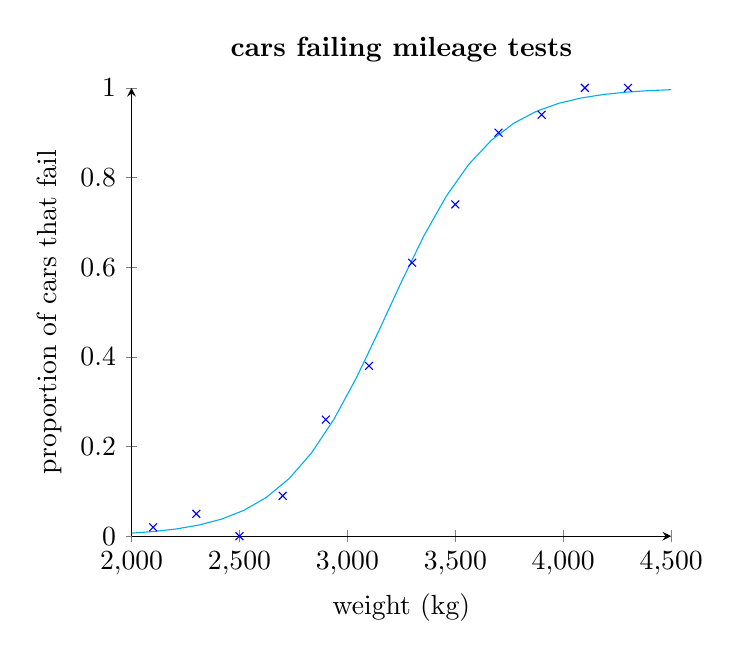
\begin{tikzpicture}
	\begin{axis}[
	xmin=2000, xmax=4500, xlabel=weight (kg),
	ymin=0, ymax=1, ylabel=proportion of cars that fail,
	title=\textbf{cars failing mileage tests},
	axis x line=bottom,
	axis y line=left,
	domain=2000:4500,
	]
	\addplot[blue, only marks, mark=x] coordinates {
		(2100.00,0.02)
		(2300.00,0.05)
		(2500.00,0.00)
		(2700.00,0.09)
		(2900.00,0.26)
		(3100.00,0.38)
		(3300.00,0.61)
		(3500.00,0.74)
		(3700.00,0.90)
		(3900.00,0.94)
		(4100.00,1.00)
		(4300.00,1.00)
	};
	\addplot[cyan] {1/(1+exp(-(-13.38 + 0.0042*x)))};
	\end{axis}
	\end{tikzpicture}
\end{center}

Unlike for linear models, we cannot read off effect sizes directly from parameter estimates in GLMs. \textcolor{red}{Need to consider the link function.}